\documentclass[11pt,]{article}
\usepackage{lmodern}
\usepackage{amssymb,amsmath}
\usepackage{ifxetex,ifluatex}
\usepackage{fixltx2e} % provides \textsubscript
\ifnum 0\ifxetex 1\fi\ifluatex 1\fi=0 % if pdftex
  \usepackage[T1]{fontenc}
  \usepackage[utf8]{inputenc}
\else % if luatex or xelatex
  \ifxetex
    \usepackage{mathspec}
    \usepackage{xltxtra,xunicode}
  \else
    \usepackage{fontspec}
  \fi
  \defaultfontfeatures{Mapping=tex-text,Scale=MatchLowercase}
  \newcommand{\euro}{€}
    \setmainfont{Georgia}
\fi
% use upquote if available, for straight quotes in verbatim environments
\IfFileExists{upquote.sty}{\usepackage{upquote}}{}
% use microtype if available
\IfFileExists{microtype.sty}{%
\usepackage{microtype}
\UseMicrotypeSet[protrusion]{basicmath} % disable protrusion for tt fonts
}{}
\usepackage[margin=1.0in]{geometry}
\ifxetex
  \usepackage[setpagesize=false, % page size defined by xetex
              unicode=false, % unicode breaks when used with xetex
              xetex]{hyperref}
\else
  \usepackage[unicode=true]{hyperref}
\fi
\hypersetup{breaklinks=true,
            bookmarks=true,
            pdfauthor={},
            pdftitle={},
            colorlinks=true,
            citecolor=blue,
            urlcolor=blue,
            linkcolor=magenta,
            pdfborder={0 0 0}}
\urlstyle{same}  % don't use monospace font for urls
\usepackage{graphicx,grffile}
\makeatletter
\def\maxwidth{\ifdim\Gin@nat@width>\linewidth\linewidth\else\Gin@nat@width\fi}
\def\maxheight{\ifdim\Gin@nat@height>\textheight\textheight\else\Gin@nat@height\fi}
\makeatother
% Scale images if necessary, so that they will not overflow the page
% margins by default, and it is still possible to overwrite the defaults
% using explicit options in \includegraphics[width, height, ...]{}
\setkeys{Gin}{width=\maxwidth,height=\maxheight,keepaspectratio}
\setlength{\parindent}{0pt}
\setlength{\parskip}{6pt plus 2pt minus 1pt}
\setlength{\emergencystretch}{3em}  % prevent overfull lines
\providecommand{\tightlist}{%
  \setlength{\itemsep}{0pt}\setlength{\parskip}{0pt}}
\setcounter{secnumdepth}{0}

%%% Use protect on footnotes to avoid problems with footnotes in titles
\let\rmarkdownfootnote\footnote%
\def\footnote{\protect\rmarkdownfootnote}

%%% Change title format to be more compact
\usepackage{titling}

% Create subtitle command for use in maketitle
\newcommand{\subtitle}[1]{
  \posttitle{
    \begin{center}\large#1\end{center}
    }
}

\setlength{\droptitle}{-2em}
  \title{}
  \pretitle{\vspace{\droptitle}}
  \posttitle{}
  \author{}
  \preauthor{}\postauthor{}
  \date{}
  \predate{}\postdate{}

\usepackage{booktabs}
\usepackage[final]{changes}
\usepackage[font={small},labelfont=bf,labelsep=colon]{caption}
\linespread{1.2}
\usepackage[compact]{titlesec}
\usepackage{enumitem}
\usepackage{tikz}
\def\checkmark{\tikz\fill[scale=0.4](0,.35) -- (.25,0) -- (1,.7) -- (.25,.15) -- cycle;}
\setlist{nolistsep}
\titlespacing{\section}{2pt}{*0}{*0}
\titlespacing{\subsection}{2pt}{*0}{*0}
\titlespacing{\subsubsection}{2pt}{*0}{*0}
\setlength{\parskip}{3pt}
\setremarkmarkup{(#2)}
\definechangesauthor[name={Nick Tustison}, color=red]{nt}
\definechangesauthor[name={James Stone}, color=magenta]{js}
\definechangesauthor[name={Lisa Wilde}, color=cyan]{lw}
\definechangesauthor[name={Andy Mayer}, color=green]{am}
\definechangesauthor[name={Harvey Levin}, color=blue]{hl}
\definechangesauthor[name={Brian Taylor}, color=purple]{bt}
\definechangesauthor[name={David Tate}, color=orange]{dt}

% Redefines (sub)paragraphs to behave more like sections
\ifx\paragraph\undefined\else
\let\oldparagraph\paragraph
\renewcommand{\paragraph}[1]{\oldparagraph{#1}\mbox{}}
\fi
\ifx\subparagraph\undefined\else
\let\oldsubparagraph\subparagraph
\renewcommand{\subparagraph}[1]{\oldsubparagraph{#1}\mbox{}}
\fi

\begin{document}
\maketitle

\pagenumbering{gobble}

\section{Abstract}\label{abstract}

White matter hyperintensities (WMHs) are foci of abnormal signal
intensity in white matter regions seen with magnetic resonance imaging
(MRI). WMHs are associated with normal aging and have shown prognostic
value in neurological conditions such as traumatic brain injury (TBI).
The impracticality of manually quantifying these lesions limits their
clinical utility and motivates the utilization of machine learning
techniques for automated segmentation workflows. Herein, we develop a
concatenated random forest framework with image features for segmenting
WMHs in a TBI cohort. The framework is built upon the Advanced
Normalization Tools (ANTs) and ANTsR toolkits. MR (3D FLAIR, T2-, and
T1-weighted) images from 24 service members and veterans scanned in the
Chronic Effects of Neurotrauma Consortium's (CENC) observational study
were acquired. Manual annotations were employed for both training and
evaluation using a leave-one-out strategy.
\textcolor{blue}{Performance measures include sensitivity,
positive predictive value, $F_1$ score, and relative volume difference.
Final average results were: sensitivity = 0.68 $\pm$ 0.38, positive
predictive value = 0.51 $\pm$ 0.40, $F_1$ = 0.52 $\pm$ 0.36,
relative volume difference} = 43 \(\pm\) 26\%. In addition, three lesion
size ranges are selected to illustrate the variation in performance with
lesion size.\} Paired with correlative outcome data, supervised learning
methods may allow for identification of imaging features predictive of
diagnosis and prognosis in individual TBI patients.

\clearpage

\section{Introduction}\label{introduction}

\subsection{White matter hyperintensities in
TBI}\label{white-matter-hyperintensities-in-tbi}

\textcolor{blue}{White matter hyperintensities (WMHs) are foci of abnormally increased signal intensity seen within white matter regions within the cerebrum and brainstem on fluid attenuation inversion recovery (FLAIR) magnetic resonance imaging (MRI) sequences.
WMHs are a frequent finding following traumatic brain injury (TBI) and have been correlated with functional outcome and injury severity in both pediatric}\textsuperscript{1,2}
\textcolor{blue}{and adult}\textsuperscript{3--6}
\textcolor{blue}{populations.}

\textcolor{blue}{Further research involving WMHs has shown that regional distribution and volume of WMHs have been shown to possess prognostic value in the TBI patient}\textsuperscript{2,6--8}\textcolor{blue}{. Specifically, lesion volume in corpus callosum correlates with functional scores in the acute phase following injury, while lesion volume in frontal lobes correlates with scores at 1 year following injury}\textsuperscript{6}\textcolor{blue}{.
Further, volume of FLAIR lesions within the corpus
callosum, brainstem, and thalamus in patients with severe TBI correlates
with Glasgow Outcome-Extended (GOS-E) scores---a numeric groupwise assessment used to
classify ``outcome'' in TBI patients where ``outcome'' refers to the
spectrum of possible prognoses from death to disability to recovery}\textsuperscript{4}\textcolor{blue}{. Additionally,
in patients who are comatose following severe TBI
the regional distribution of FLAIR lesions within the pons, midbrain, hypothalamus, basal forebrain, parietal, temporal, occipital lobes, and insula along with the observation of grasping or chewing behavior are associated with poor outcome}\textsuperscript{7}.

\textcolor{blue}{Despite the above findings which demonstrate that WMHs have potential prognostic value, they are not routinely employed as a diagnostic measure in clinical practice.  Performing a comprehensive manual counting of number and distribution of lesions in the clinical setting is simply not practical. The development of such lesion quantification approaches may allow for the practical inclusion of this type of information within routine radiological practice.  In this work, we present an automated framework for quantification of WMHs in
multi-modal MRI using the random forest machine learning technique.}

\subsection{Random forests for WMH
segmentation}\label{random-forests-for-wmh-segmentation}

The random forests framework\textsuperscript{9} is a popular machine
learning technique that has demonstrated significant utility for
supervised segmentation tasks (e.g., normal human brain
segmentation\textsuperscript{10}) and other computer vision applications
(e.g.,\textsuperscript{11}).
\textcolor{blue}{Random forest-based paradigms have been successfully employed in the
delineation of other neuropathologies}\textsuperscript{12--17}
\textcolor{blue}{for both single and multi-modal acquisition protocols.}

Random forests are conceptually straightforward\textsuperscript{9}.
\textcolor{blue}{The basic component of
the random forest paradigm is the ``decision tree'' often represented by a flowchart or
graph where internal nodes represent ``tests'', or decisions, and the edges represent the outcome of those tests.  The final, or end, nodes represent the various classsifications produced by traversal through the decision tree.  For the proposed application, individual
voxels (and their corresponding feature values) are introduced at the root of a particular
decision tree and traverse the edges and internal nodes ultimately ending up at one of
the classification nodes according to the tests at each internal node.  A single random
forest model will consist of many such trees (often refered to as an ``ensemble'').}
\textcolor{blue}{Although decision trees had been extensively studied, the success of employing collections of such weak learners for boosting machine learning performance
(e.g., AdaBoost)}\textsuperscript{18,19}
\textcolor{blue}{influenced the similarly sytled conglomeration of decision trees into ``forests'' with randomized node optimization}\textsuperscript{20,21}.
\textcolor{blue}{Finally, Breiman}\textsuperscript{9}
\textcolor{blue}{improved accuracy by random sampling of training data (i.e., ``bagging'') resulting
in the current random forest technique applied here.}
\textcolor{blue}{As voxels and their feature values are ``pushed'' through each decision tree in the forest,  votes for each label are accumulated and converted to probability values for all classification possiblilities at
each voxel location.}

In this work, we develop a concatenated random forest framework with a
feature image set (both spatial and intensity-based) for segmenting WMHs
in a large TBI cohort. The entire framework is built on the well-known
open-source Advanced Normalization Tools (ANTs)\footnote{\url{https://github.com/stnava/ANTs}}
and ANTsR\footnote{\url{https://github.com/stnava/ANTsR}} toolkits.
Further motivating this research is the availability of several large
publicly available imaging data sets that permits testing
reproducibility of this automated routine for WMH segmentation and
quantification.

\section{Materials and Methods}\label{materials-and-methods}

\subsection{Imaging}\label{imaging}

MR images utilized for this initial report were acquired from a single
scanner involved in the Chronic Effects of Neurotrauma Consortium's
(CENC) observational study (see Walker et al., this issue). Briefly,
participants were Operation Iraqi Freedom/Operation Enduring Freedom
(OIF/OEF) era Service Members and Veterans between the ages of 18-60
years with prior combat exposure and deployment(s). The feature images
\textcolor{blue}{were derived from MR acquisitions of} 26 subjects aged
39.6 \(\pm\) 8.1 years (range 28--58 years). Within this cohort, 24
(92\%) were considered positive for TBI based upon the potential
concussive events (PCE) interview process described in detail in Walker
et al., this issue).
\textcolor{blue}{All lesions were isolated in the white matter of the cerebrum.  Table 1 provides a descriptive statistical summary of the variation in lesion
load across the selected cohort.}

\begin{table}[!htb]
  \centering
  \begin{tabular*}{1.0\textwidth}{@{\extracolsep{\fill}} rrrrr}
    \textbf{Subject id} & \textbf{Lesion count} & \textbf{Lesion load} & \textbf{Mean volume} & \textbf{[Min $-$ Max]} \\
    \toprule
    \midrule
    0 & 2 & 18 & 9 $\pm$ 1.4 & [8-10] \\
    1 & 3 & 3 & 1 $\pm$ 0 & [1-1] \\
    2 & 0 & 0 & 0 & [0-0] \\
    3 & 11 & 209 & 19 $\pm$ 18.4 & [1-56] \\
    4 & 3 & 130 & 43.3 $\pm$ 50.0 & [12-101] \\
    5 & 1 & 2 & 2 & [2-2] \\
    6 & 25 & 790 & 31.6 $\pm$ 29.2 & [2-132] \\
    7 & 24 & 767 & 32.0 $\pm$ 33.6 & [2-166] \\
    8 & 3 & 18 & 6 $\pm$ 7.8 & [1-15] \\
    9 & 21 & 508 & 24.2 $\pm$ 35.1 & [1-166] \\
    10 & 2 & 17 & 8.5 $\pm$ 10.6 & [1-16] \\
    11 & 7 & 151 & 21.6 $\pm$ 21.7 & [1-61] \\
    12 & 46 & 901 & 19.6 $\pm$ 17.9 & [1-115] \\
    13 & 1 & 1 & 1 & [1-1] \\
    14 & 2 & 32 & 16 $\pm$ 9.9 & [9-23] \\
    15 & 2 & 22 & 11 $\pm$ 14.1 & [1-21] \\
    16 & 8 & 124 & 15.5 $\pm$ 8.4 & [6-34] \\
    17 & 3 & 140 & 46.7 $\pm$ 53.1 & [1-105] \\
    18 & 3 & 10 & 3.3 $\pm$ 4.0 & [1-8] \\
    19 & 20 & 784 & 39.2 $\pm$ 63.2 & [1-230] \\
    20 & 3 & 6 & 2 $\pm$ 1.7 & [1-4] \\
    21 & 7 & 244 & 34.9 $\pm$ 32.3 & [1-93] \\
    22 & 12 & 236 & 19.7 $\pm$ 13.5 & [1-52] \\
    23 & 63 & 4078 & 64.7 $\pm$ 93.6 & [1-551] \\
    \midrule
    Total & 272 & 9191 & 33.8 $\pm$ 55.4 & [1-551] \\
    \midrule
    \bottomrule
  \end{tabular*}
\label{table:trainingData}
\caption{Descriptive lesion statistics for the cohort used for the evaluation.
         Lesion load, mean volume ($\pm$ standard deviation), and the min/max range are given in terms of
         the number of voxels
         since all image acquisitions were performed with the same image
         voxel resolution ($1\times1\times1.2$ mm$^3$).
         }
\end{table}


Images were acquired on a Philips 3.0T Ingenia system with an 8-channel
SENSE head coil (Philips Medical Systems, Best, Netherlands). 3D FLAIR
sequences were acquired with a turbo spin echo inversion recovery
sequence with the following parameters: repetition time (TR) = 4800 ms,
echo time (TE) = 325 ms, inversion time (TI) = 1650 ms; 170 sagittal
slices with a 1.2 mm slice thickness, 256 \(\times\) 256 acquisition
matrix, and 256 \(\times\) 256 mm FOV. 3D T1-weighted sequences were
acquired with a fast field echo (FFE) sequence with the following
parameters: TR = 6.8 ms, TE = 3.2 ms, echo train length (ETL) = 240;
Flip angle = 9\(^\circ\), 170 sagittal slices with a 1.2 mm slice
thickness, 256x240 acquisition matrix, and 256 \(\times\) 256 mm FOV. In
addition, 3D T2-weighted images were acquired with a turbo spin echo
sequence with the following parameters: TR = 2500 ms, TE = 245 ms, ET: =
133; 170 sagittal slices with a 1.2 mm slice thickness, 256 \(\times\)
256 acquisition matrix, and 256 x 256 mm FOV.

\textcolor{blue}{The first author (J. R. S.) performed the manual WMH tracings for all 26
subjects.  J. R. S. is a radiologist certified by the American Board of Radiology, with a certificate of advanced qualification in vascular and interventional radiology, over 18 years of research experience in TBI, and 6 years of clinical imaging experience.  All
multi-modal MR dicom image slices were converted to the nifti file format}.\footnote{\url{http://nifti.nimh.nih.gov/nifti-1}}
\textcolor{blue}{All nifti image volumes for each subject were rigidly aligned to the T1 image of that subject using the ANTs software}\textsuperscript{22}
\textcolor{blue}{.  The normalized MRI volumes were then provided to
J. R. S. who traced each lesion using the ITK-SNAP tool}\textsuperscript{23}
\textcolor{blue}{
which has multi-image overlay capabilities for visualizing all modalities in all three
canonical views.}

\subsection{Quantitative analysis}\label{quantitative-analysis}

\textcolor{blue}{Figure 1 provides a graphical overview of the proposed workflow.  The major components
include offline generation of symmetric multimodal templates, the creation of
feature images from the training data which are then employed for statistical
prediction using a concatenated random forest framework.  This framework involves
the use of two random forest models where the outcome (i.e., the tissue
probability estimates) of the first RF model application,
which we denote as ``Stage1'', is used as input (along with the original set of
feature images) to a refinement RF model segmentation which we denote as ``Stage 2''.
Once these offline steps
are performed, a new (i.e., unsegmented) subject can then be processed using the proposed pipeline.}

\begin{figure}[htbp]
\centering
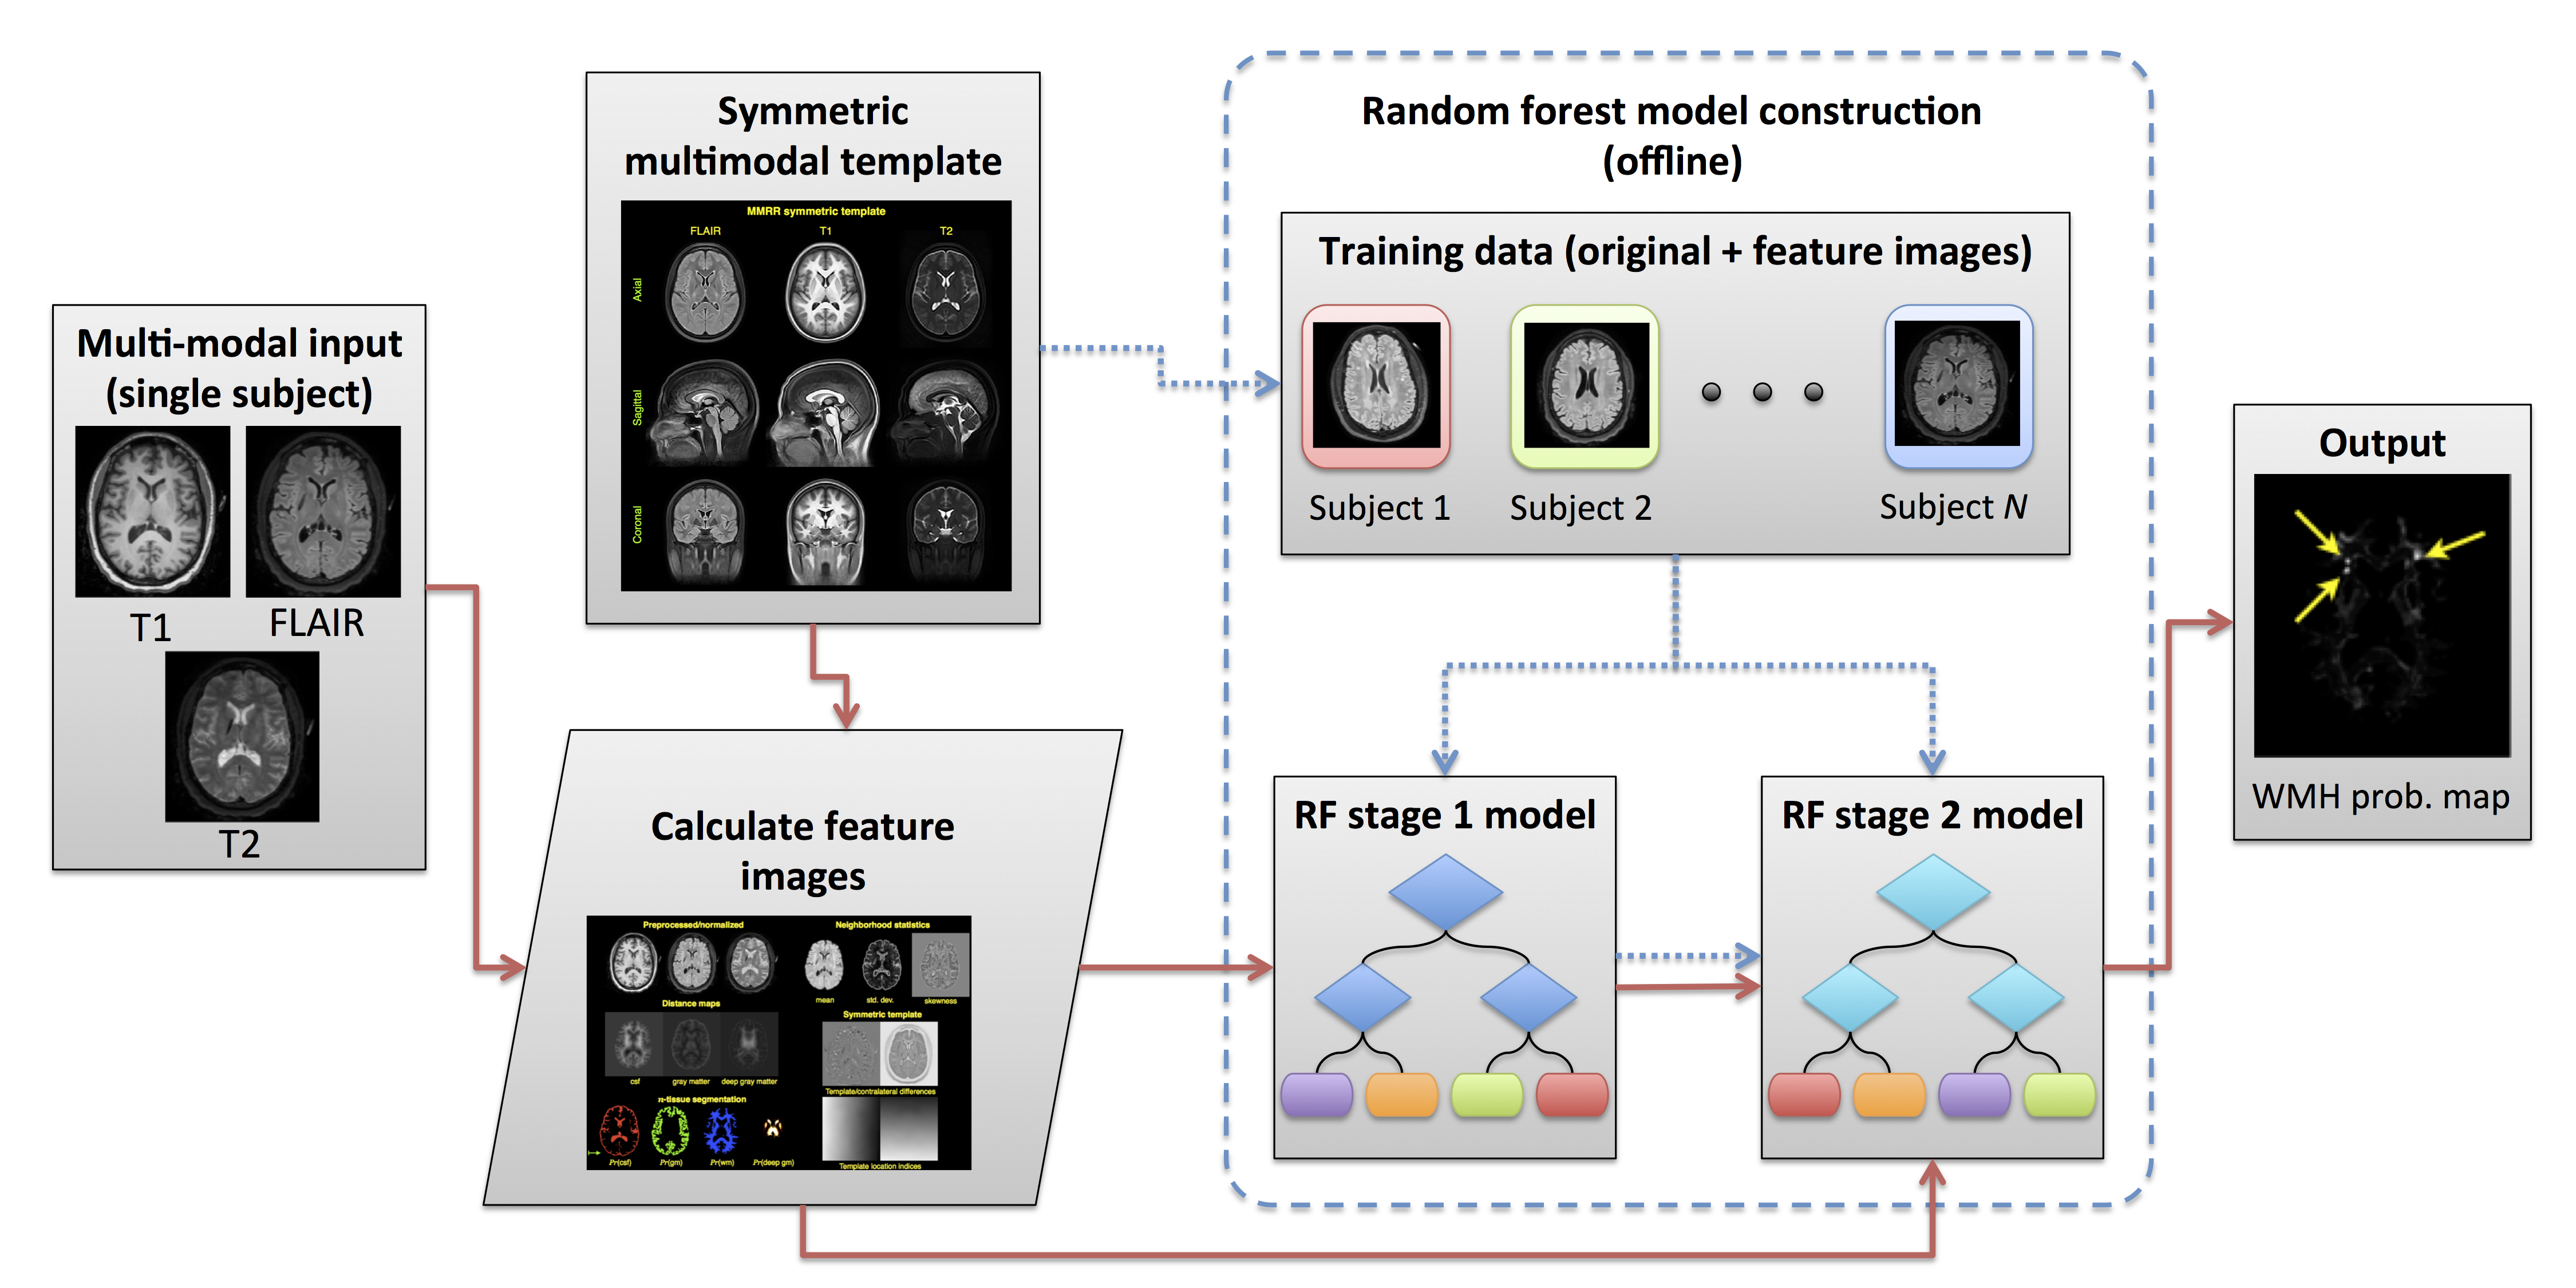
\includegraphics{Figures/wmhPipeline.png}
\caption{\textcolor{blue}{Workflow illustration for the proposed pipeline.  Processing of the multi-modal
input MRI for a single subject, using the multi-modal symmetric template, results in
the generation of the feature images.  These feature images are used as input to the
Stage 1 RF model producing the initial RF probability map estimates.  The Stage 1
voting maps, the original feature images, and the Stage 2 RF model result in the
final voting maps which includes the WMH probability estimate.  Note that the RF models
are constructed once from a set of training data which are processed using the
same feature-construction pipeline as the single-subject input MRI.}}
\end{figure}

\subsubsection{Symmetric multi-modal
templates}\label{symmetric-multi-modal-templates}

\textcolor{blue}{Following}\textsuperscript{24}
\textcolor{blue}{and}\textsuperscript{17},
\textcolor{blue}{optimally derived templates
serve for both brain tissue segmentation (for the derivation of tissue prior probability maps) and generation of asymmetry feature images.
For this work we use the multi-modal data available from the public MMRR data set}\textsuperscript{25}\textcolor{blue}{.  We used all 46 multi-modal acquisitions of that study to produce a multi-modal template according to the procedure described in}\textsuperscript{26}
\textcolor{blue}{which
results in a mean (in terms of both shape and intensity) multivariate template representing the entire cohort.  Mid-canonical slices of the FLAIR, T1, and T2 components are illustrated in Figure 2.}

\begin{figure}[htbp]
\centering
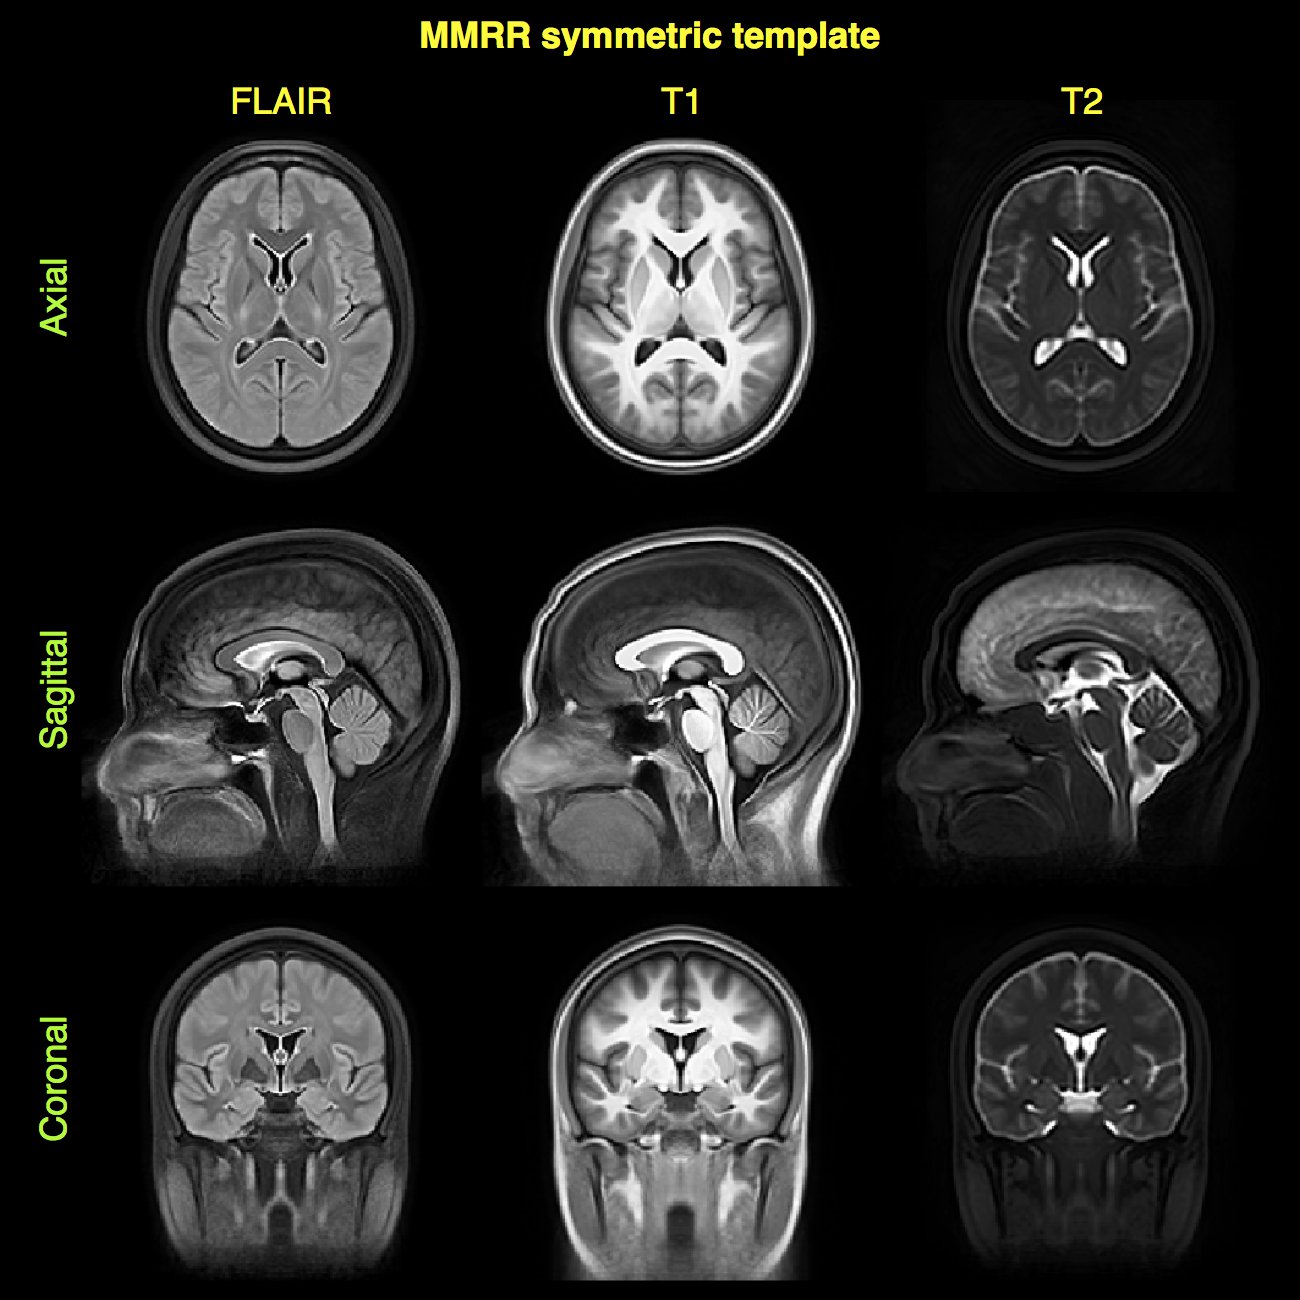
\includegraphics{Figures/MMRR.png}
\caption{Canonical views of the mutlivariate, bilaterally symmetric
template constructed from the MMRR data set\textsuperscript{25} (only
shown are the FLAIR, T1, and T2 modalities--- the components relevant
for this work). Template construction is detailed
in\textsuperscript{17}. These images are important for specific
asymmetry-based features.}
\end{figure}

\subsubsection{Feature images for WMH
segmentation}\label{feature-images-for-wmh-segmentation}

\textcolor{blue}{
Crucial to these supervised segmentation approaches are the creation and selection of
``features'' as input (i.e., feature images constructed from the training data)
in conjunction with expertly identified structures of interest
(i.e., WMHs) for model construction.} For the targeted application in
this work, tissue classification is performed at the voxelwise level. In
other words, each voxel within the region of interest is sent through
the ensemble of decision trees and receives a set of classification
votes from each tree thus permitting a regression or classification
solution. Since this procedure is performed at the voxelwise level,
intensity information alone is insufficient for good segmentation
performance due to the lack of spatial context. For example, as pointed
out in\textsuperscript{27}, higher intensities can be found at the
periventricular caps in normal subjects which often confounds automated
lesion detection algorithms. Other potential confounds include MR signal
inhomogeneity and noise. Therefore, even though machine learning and
pattern recognition techniques are extremely powerful and have
significant potential, just as crucial to outcome is the creative
construction and deployment of salient feature images which we detail
below.

\begin{table}[!htb]
  \centering
  \begin{tabular*}{0.65\textwidth}{@{\extracolsep{\fill}} ll}
    \multicolumn{1}{c}{\textbf{Feature type}} & \multicolumn{1}{c}{\textbf{Image source}} \\
    \toprule
    \midrule
    \multicolumn{2}{c}{\textbf{Intensities}} \\
    \midrule
    normalized/preprocessed & FLAIR, T1, and T2 \\
    \midrule
    \multicolumn{2}{c}{\textbf{Symmetric template}} \\
    \midrule
    template difference & FLAIR, T1, and T2 \\
    contralateral difference & FLAIR, T1, and T2 \\
    location indices & FLAIR, T1, and T2 \\
    \midrule
    \multicolumn{2}{c}{\textbf{Segmentation probabilities}} \\
    \midrule
    $Pr$(cerebrospinal fluid) & T1 \\
    $Pr$(gray matter) & T1 \\
    $Pr$(white matter) & T1 \\
    $Pr$(deep bray matter) & T1 \\
    $Pr$(brain stem) & T1 \\
    $Pr$(cerebellum) & T1 \\
    \midrule
    \multicolumn{2}{c}{\textbf{Distance maps}} \\
    \midrule
    cerebrospinal fluid & T1 brain segmentation \\
    gray matter & T1 brain segmentation \\
    deep gray matter & T1 brain segmentation \\
    whole brain & T1 brain segmentation \\
    \midrule
    \multicolumn{2}{c}{\textbf{Neighborhood statistics}} \\
    \midrule
    mean & FLAIR, T1, and T2 \\
    standard deviation & FLAIR, T1, and T2 \\
    skewness & FLAIR, T1, and T2 \\
    \midrule
    \bottomrule
  \end{tabular*}
 \label{table:indices}
 \caption{List of feature images used for Stage 1 of the proposed white matter
          hyperintensity segmentation framework.}
\end{table}




Supervised methodologies are uniquely characterized, in part, by the
feature images that are used to identify the regions of interest. In
Table 2, we provide a list and basic categorization of the feature
images used for the initial (i.e., Stage 1---more on the use of multiple
random forest stages below) segmentation of the WMHs. In addition Figure
3 provides a representation of a set of feature images for a single
subject analyzed in this work. Note that in this work we categorize the
brain parenchyma with seven labels:

\begin{itemize}
\tightlist
\item
  cerebrospinal fluid (label 1),
\item
  gray matter (label 2),
\item
  white matter (label 3),
\item
  deep gray matter (label 4),
\item
  brain stem (label 5),
\item
  cerebellum (label 6), and
\item
  white matter hyperintensities (label 7).
\end{itemize}

\begin{figure}[htbp]
\centering
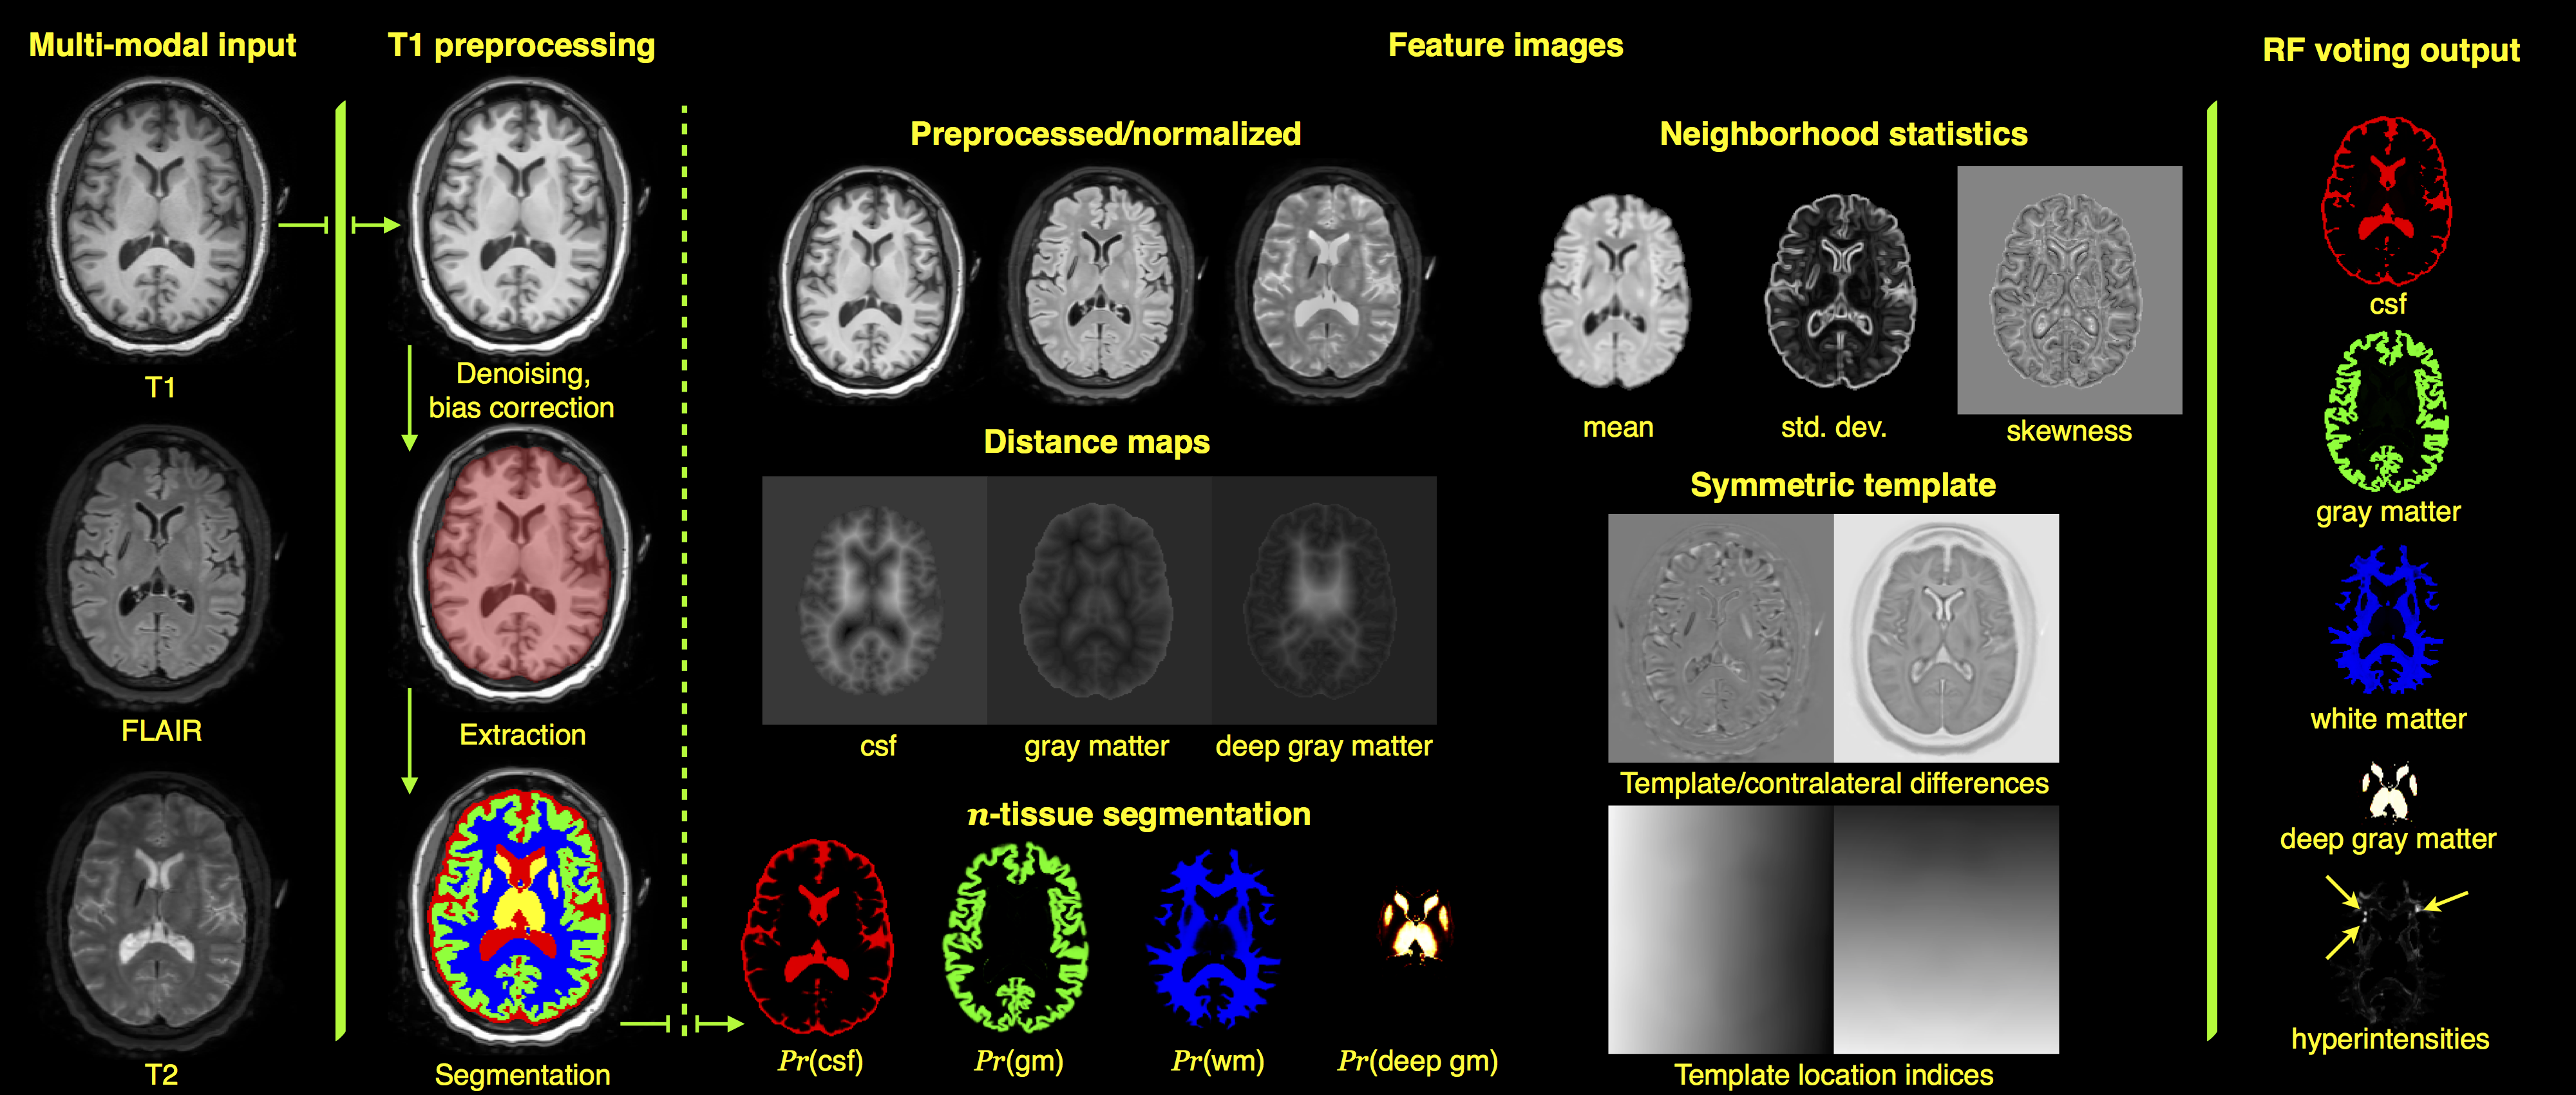
\includegraphics{Figures/featureImages.png}
\caption{Representation of Stage 1 feature images for subject 01C1019.
The FLAIR, T1-, and T2-weighted images are rigidly
pre-aligned\textsuperscript{22} to the space of the FLAIR image. The
three modality images are then preprocessed (N4 bias
correction\textsuperscript{28} and adaptive
denoising\textsuperscript{29}) followed by application of standard ANTs
brain extraction and \(n\)-tissue segmentation protocols using the MMRR
symmetric template and corresponding priors\textsuperscript{24} applied
to the T1 image. The feature images are then generated for voxelwise
input to the RF model which results in the voting maps illustrated on
the right. This gives a probabilistic classification of tissue type. Not
shown are the probability and voting images for the brain stem and
cerebellum.}
\end{figure}

As mentioned previously, input for each subject comprises FLAIR, T1-,
and T2-weighted acquisitions. The T1 and T2 images are rigidly
registered to the FLAIR image using the open-source Advanced
Normalization Tools (ANTs)\textsuperscript{22}. The aligned images are
then preprocessed using the denoising algorithm of\textsuperscript{29}
followed by N4 bias correction\textsuperscript{28} which are then
normalized to the intensity range \([0,1]\). Although we could have used
an alternative intensity standardization algorithm
(e.g.,\textsuperscript{30}), we found that a simple linear rescaling
produced better results similar to previous work\textsuperscript{17}.

\begin{figure}[htbp]
\centering
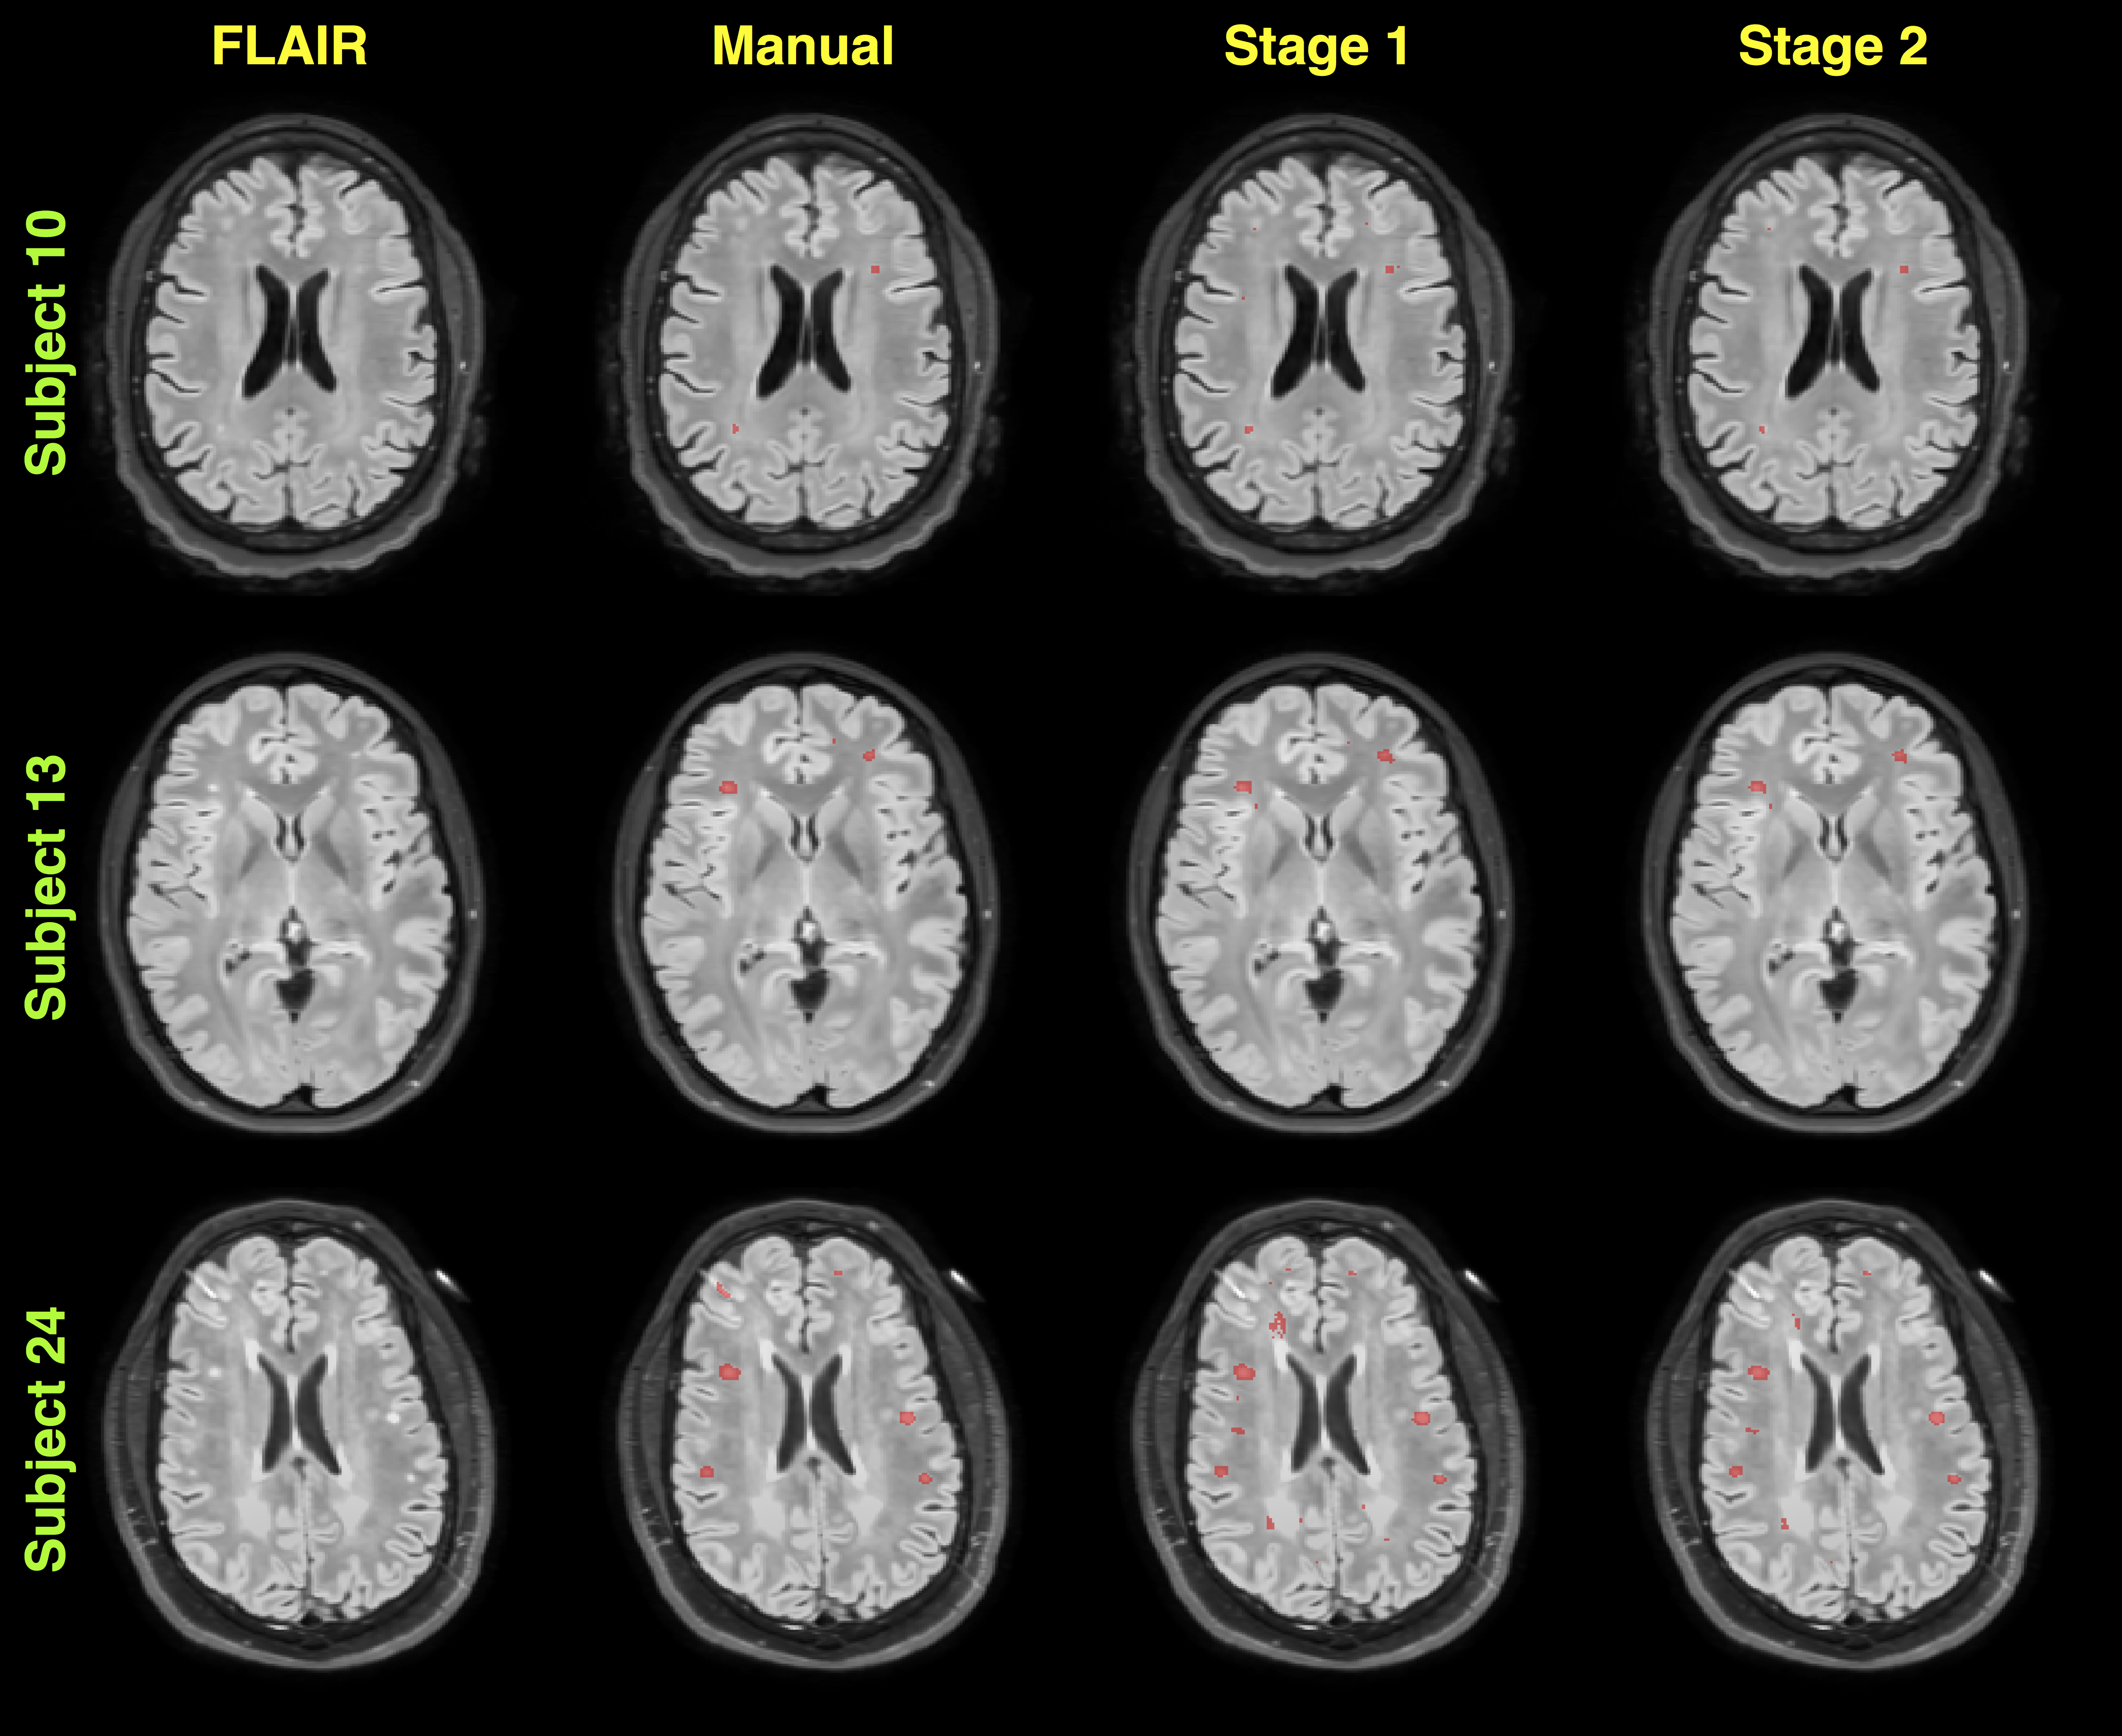
\includegraphics{Figures/sampleResults.png}
\caption{Sample FLAIR acquisition image slices showing both manual and
random forest segmentations for both stages obtained during the
leave-one-out evaluation. Manual segmentations were performed by one of
the authors and provided the ground truth WMH labels for training the
random forest models.}
\end{figure}

The T1 image is then processed via the ANTs brain extraction and normal
tissue segmentation pipelines\textsuperscript{24}. The result is a mask
delineating the brain parenchyma and probabilistic estimates of the CSF,
gray matter, white matter, deep gray matter, brain stem, and
cerebellum\textsuperscript{31}. These provide the expertly annotated
labels for the first six tissue labels given above. Tissue prior
probability maps for segmentation are from multi-model optimal symmetric
shape/intensity templates\textsuperscript{17} created from the public
MMRR data set\textsuperscript{25} (cf Figure 2).

Feature values include the preprocessed FLAIR, T1, and T2 image voxel
intensities. We also calculate a set of neighborhood statistics (mean,
standard deviation, and skewness) feature images using a Manhattan
radius of one voxel given the typical size of individual WMHs. For each
of the preprocessed images, we calculate the difference in intensities
with the corresponding warped template component. Previous success in
the international brain tumor segmentation
competition\textsuperscript{32} was based on an important set of
intensity features that were created from multi-modal templates
mentioned previously\textsuperscript{17} and listed in Table 2. We
employ the same strategy here.

To take advantage of the gross bilateral symmetry of the normal brain
(in terms of both shape and intensity), and the fact that WMHs do not
generally manifest symmetrically across hemispheres, we use the
symmetric templates to compute the contralateral intensity differences
as an additional intensity feature.

The segmentation probability images described above are used as feature
images to provide a spatial context for the random forest model
prediction step. Additional spatial contextual feature images include
the distance maps\textsuperscript{33} based on the csf, gray matter, and
deep gray matter images. These latter images are intended to help
distinguish white matter hyperintensities from false positives induced
by the partial voluming at the gray/white matter interface. A third set
of images are based on the voxel location within the space of the
template.
\textcolor{blue}{Similar feature images were used in}\textsuperscript{34}
\textcolor{blue}{although, unlike the proposed framework, this previous work lacks
normalization to the standard
coordinate system provided by the template to dramatically improve spatial specificity
across all subjects.  To generate these images, the T1 image of each subject is
registered to the T1 template component using a B-spline variant}\textsuperscript{35}
\textcolor{blue}{of the well-known ANTs Symmetric Normalization (SyN) algorithm}\textsuperscript{36}.
\textcolor{blue}{Using the derived transforms, the template coordinate images are warped back to the space of the individual subject.}

\subsubsection{Stacked (concatenated) random forests for improved
segmentation
performance}\label{stacked-concatenated-random-forests-for-improved-segmentation-performance}

In previous brain tumor segmentation work\textsuperscript{17}, it was
demonstrated that a concatenated supervised approach, whereby the
prediction output from the first random forest model serves as partial
input for a second random forest model, can significantly improve
segmentation performance. We do the same thing for the work described
here where we employ two stacked random forests (or two ``stages''). The
Stage 1 feature images of the training data (as described previously)
are used to construct the Stage 1 model. The training data Stage 1
features are then used to produce the voxelwise ``voting maps'' (i.e.,
the classification count of each decision tree for each tissue label)
via the Stage 1 random forest model. All the Stage 1 features plus the
Stage 1 voting maps are used as input to the Stage 2 model. In addition,
we use the Stage 1 voting maps as tissue priors (i.e., probabilistic
estimates of the tissue spatial locations) for a second application of
the \(6\)-tissue segmentation algorithm with an additional Markov Random
Field spatial prior (MAP-MRF)\textsuperscript{31}.
\textcolor{blue}{In order to maximize the spatial information for the $n$-tissue segmentation process following the voxelwise RF classification of Stage 1, we use
all three aligned preprocessed images for multivariate segmentation during the
second stage.} The resulting seven posterior probability images
constitute a third additional feature image set for Stage 2.

\subsubsection{Implementation}\label{implementation}

As pointed out in a recent comprehensive lesion segmentation
review\textsuperscript{37}, although the number of algorithms reported
in the literature is quite extensive, there were only four publicly
available segmentation algorithms at the time of writing this article.
In contrast to the current work, none are based on supervised learning.
As we did for our brain tumor segmentation
algorithm\textsuperscript{17}, all of the code described in this work is
publicly available through the open-source ANTs/ANTsR toolkits. Through
ANTsR (an add-on toolkit which, in part, bridges ANTs and the R
statistical project) we use the \emph{randomForest}
package\textsuperscript{38} using the default settings with 2000 trees
per model and 500 randomly selected samples per label per image. Note
that we saw little variation in performance when these parameters were
changed (i.e.~up to 1000 random samples and as little as 1000 trees)
which is consistent with our previous experience.

In addition, similar to our previous offering,\footnote{\url{https://github.com/ntustison/ANTsAndArboles}}
we plan on creating a self-encapsulated example to showcase the proposed
methodology
\textcolor{blue}{which will also be available on github.}\footnote{\url{https://github.com/ntustison/WatchMeHyperventilate}}
The fact that the data will also be made available through the Federal
Interagency Traumatic Brain Injury Research (FITBIR) repository along
with the manual labelings will facilitate reproducibility on the part of
the reader as well as any interest in extending the proposed framework
to other data sets.

\subsubsection{Evaluation protocol
overview}\label{evaluation-protocol-overview}

In order to evaluate the protocol described, we performed a
leave-one-out evaluation using the data acquired from the 24 subjects
described above. Initial processing included the creation of all Stage 1
feature images for all subjects. The initial brain segmentation of each
T1 image and the manual white matter hyperintensity tracings were
combined to provide the truth labels for the training data. The
``truth'' labels are the seven anatomical regions given above.

The leave-one-out procedure is as follows:

\begin{itemize}
\tightlist
\item
  Create Stage 1 feature images for all 24 subjects.
\item
  For each of the 24 subjects:

  \begin{itemize}
  \tightlist
  \item
    sequester the current subject and corresponding feature images.
  \item
    construct the Stage 1 random forest model from the remaining 23
    subjects.
  \item
    apply the Stage 1 random forest model to the feature images of the
    23 training subjects.
  \item
    the previous step produces the Stage 1 voting maps for all seven
    labels.
  \item
    for each of the 23 subjects, perform a Bayesian-based segmentation
    with an MRF spatial prior using the seven voting maps as additional
    tissue priors.
  \item
    construct the Stage 2 random forest model from all the Stage 1
    feature images, seven voting maps, and seven posterior probability
    maps from the previous step.
  \item
    send the sequestered subject through the random forest models for
    both stages.
  \item
    compare the final results with the manually-defined white matter
    hyperintensity regions.
  \end{itemize}
\end{itemize}

\textcolor{blue}{Several measures have been employed in the literature for evaluating
automated white matter lesion segmentation involving such quantities as lesion load,
voxel-based overlap measures (such as the Dice similarity coefficient), and lesion-based measures.}\textsuperscript{37}\textcolor{blue}{.  For this work, due to the relatively small-size distribution}
\textcolor{blue}{of the lesion load in our data cohort (see Table 1), we used
four lesion-based measures:  sensitivity, positive predictive value (i.e., precision), $F_1$ score, and relative volume difference.  The first three quantities are based on the number of false positives ($TN$, false negatives ($FN$), and true positives ($TP$) in terms of identified lesions.  It should be noted that the number of true negatives is not readily
incorporated into measures of accuracy as the quantity of ``true negatives'' (i.e., correctly identified normal brain tissue) would severely skew accuracy assessments. The $F_1$ score is an assessment of accuracy which takes into account both the sensitivity,}

\[ sensitivity =  \frac{ TP }{TP + FN}, \]

\textcolor{blue}{and the positive predictive value (PPV),}

\[ PPV =  \frac{ TP }{TP + FP}, \]

\textcolor{blue}{such that $F_1$ is given by}

\[ F_1 =  \frac{ 2 \cdot TP }{ 2 \cdot TP + FP + FN}. \]

\textcolor{blue}{The relative volume difference is calculated for each of the true positive lesions using
the manual and predicted lesion volumes:}

\[ Relative\,\,volume\,\,difference = \frac{V_{manual} - V_{predicted}}{V_{manual}}. \]

\textcolor{blue}{To illustrate how the performance of our framework varies with lesion size, we calculated
the above measures based on evenly split quantiles of the manual estimates of lesion volumes into 3 groups.  These three size ranges (in terms of the number of voxels) are:}

\begin{itemize}
\item
  \textcolor{blue}{Quantile 1: $[1-12)$,}
\item
  \textcolor{blue}{Quantile 2: $[12-28)$, and}
\item
  \textcolor{blue}{Quantile 3: $[28-551]$}.
\end{itemize}

\textcolor{blue}{These quantiles are used to showcase the performance (cf Figure 5).}

\section{Results}\label{results}

\subsection{White matter hyperintensity segmentation
evaluation}\label{white-matter-hyperintensity-segmentation-evaluation}

\textcolor{blue}{In Figure 5 we provide the segmentation evaluations derived from the leave-one-out evaluation
of the previously described TBI data over the three lesion volume ranges.
These performance measures include sensitivity,
positive predictive value, $F_1$ score, and relative volume difference.  The three lesion
size ranges over which these measures are computed are meant to illustrate the variation
in performance with lesion size.}

\textcolor{blue}{Smaller lesions ($< 12$ voxels) are more difficult
to identify which is why the sensitivity for this range is more varied compared with the largest
set of lesions ($> 28$ voxels).   The first three measures are based on the identification of
entire lesions.  The relative volume difference provides a direct assessment of the accuracy of
the volumetric estimate when comparing the manually identified lesions versus the
automatically predicted lesions.}

\textcolor{blue}{
We averaged these measures over all lesions and all subjects which resulted in the
following values:}

\begin{itemize}
\item
  \textcolor{blue}{Stage 1}

  \begin{itemize}
  \item
    \textcolor{blue}{sensitivity} = 0.70 \(\pm\) 0.34
  \item
    \textcolor{blue}{PPV} = 0.42 \(\pm\) 0.36
  \item
    \textcolor{blue}{$F_1$} = 0.47 \(\pm\) 0.36
  \item
    \textcolor{blue}{relative volume difference} = 43 \(\pm\) 38\%
  \end{itemize}
\item
  \textcolor{blue}{Stage 1}

  \begin{itemize}
  \item
    \textcolor{blue}{sensitivity} = 0.68 \(\pm\) 0.38
  \item
    \textcolor{blue}{PPV} = 0.51 \(\pm\) 0.40
  \item
    \textcolor{blue}{$F_1$} = 0.52 \(\pm\) 0.36
  \item
    \textcolor{blue}{relative volume difference} = 43 \(\pm\) 26\%
  \end{itemize}
\end{itemize}

\begin{figure}[htbp]
\centering
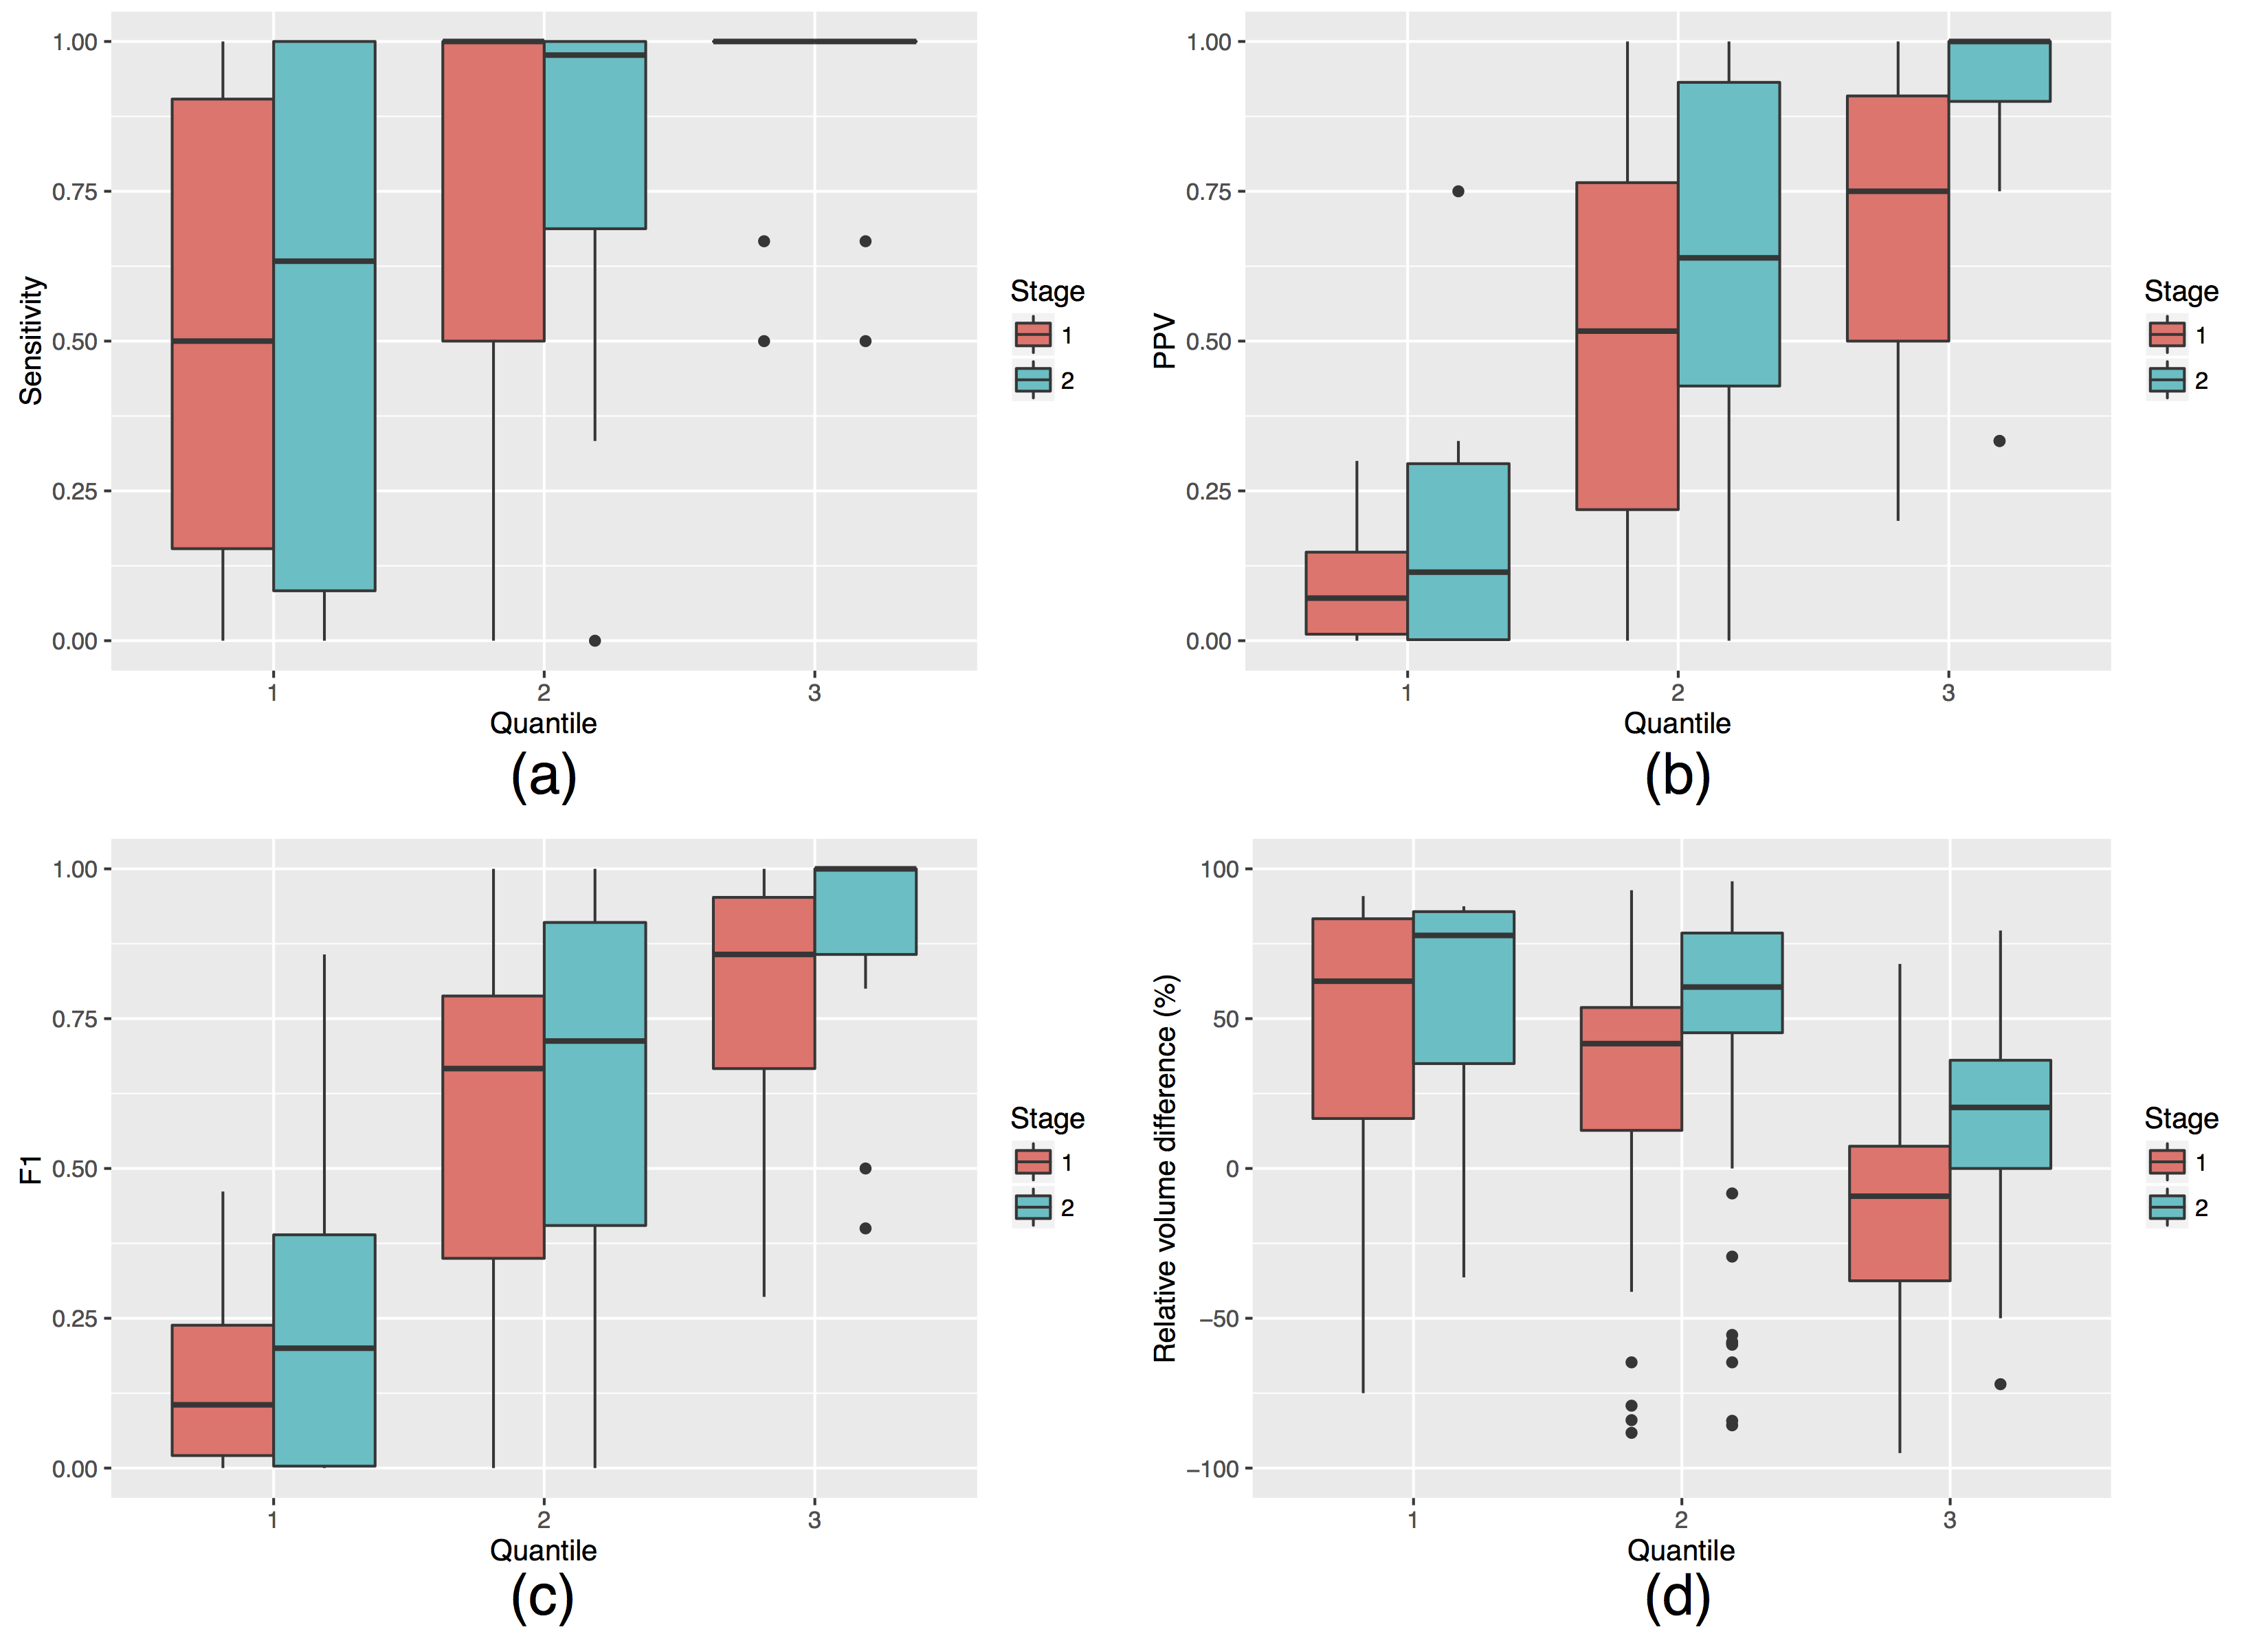
\includegraphics{Figures/evaluationResults.png}
\caption{\textcolor{blue}{Evaluation measures for both Stages of the leave-one-out protocol of the described protocol in the Methods
section:  (a) sensitivity, (b) positive predictive value, (c) $F_1$ score, and (d) relative
volume difference.   These quantitative assessments are given for three quantile ranges
spanning the range of the manually-derived lesion volumes.    Overall improvement in all
three whole lesion-based measuers is seen as the
second Stage RF model is applied for all three quantile ranges.
The relative volume difference corresponding to the Stage 2 results tend to predict a
decreased predicted volume over the Stage 1 results.}}
\end{figure}

\subsection{Ranking feature
importance}\label{ranking-feature-importance}

After performing the leave-one-out evaluation, we calculated the
\emph{MeanDecreaseAccuracy} feature values for each of the 24 subjects
\(\times\) 2 models per subject \(=48\) total models. This measure (per
feature, per model) is calculated during the out-of-bag phase of the
random forest model construction and quantifies the decrease in
prediction accuracy from omitting the specified feature. In other words,
this quantity helps determine the importance of a particular feature
and, although we save such efforts for future work, this information
provides us with guidance for future feature pruning and/or additions.

\begin{figure}[htbp]
\centering
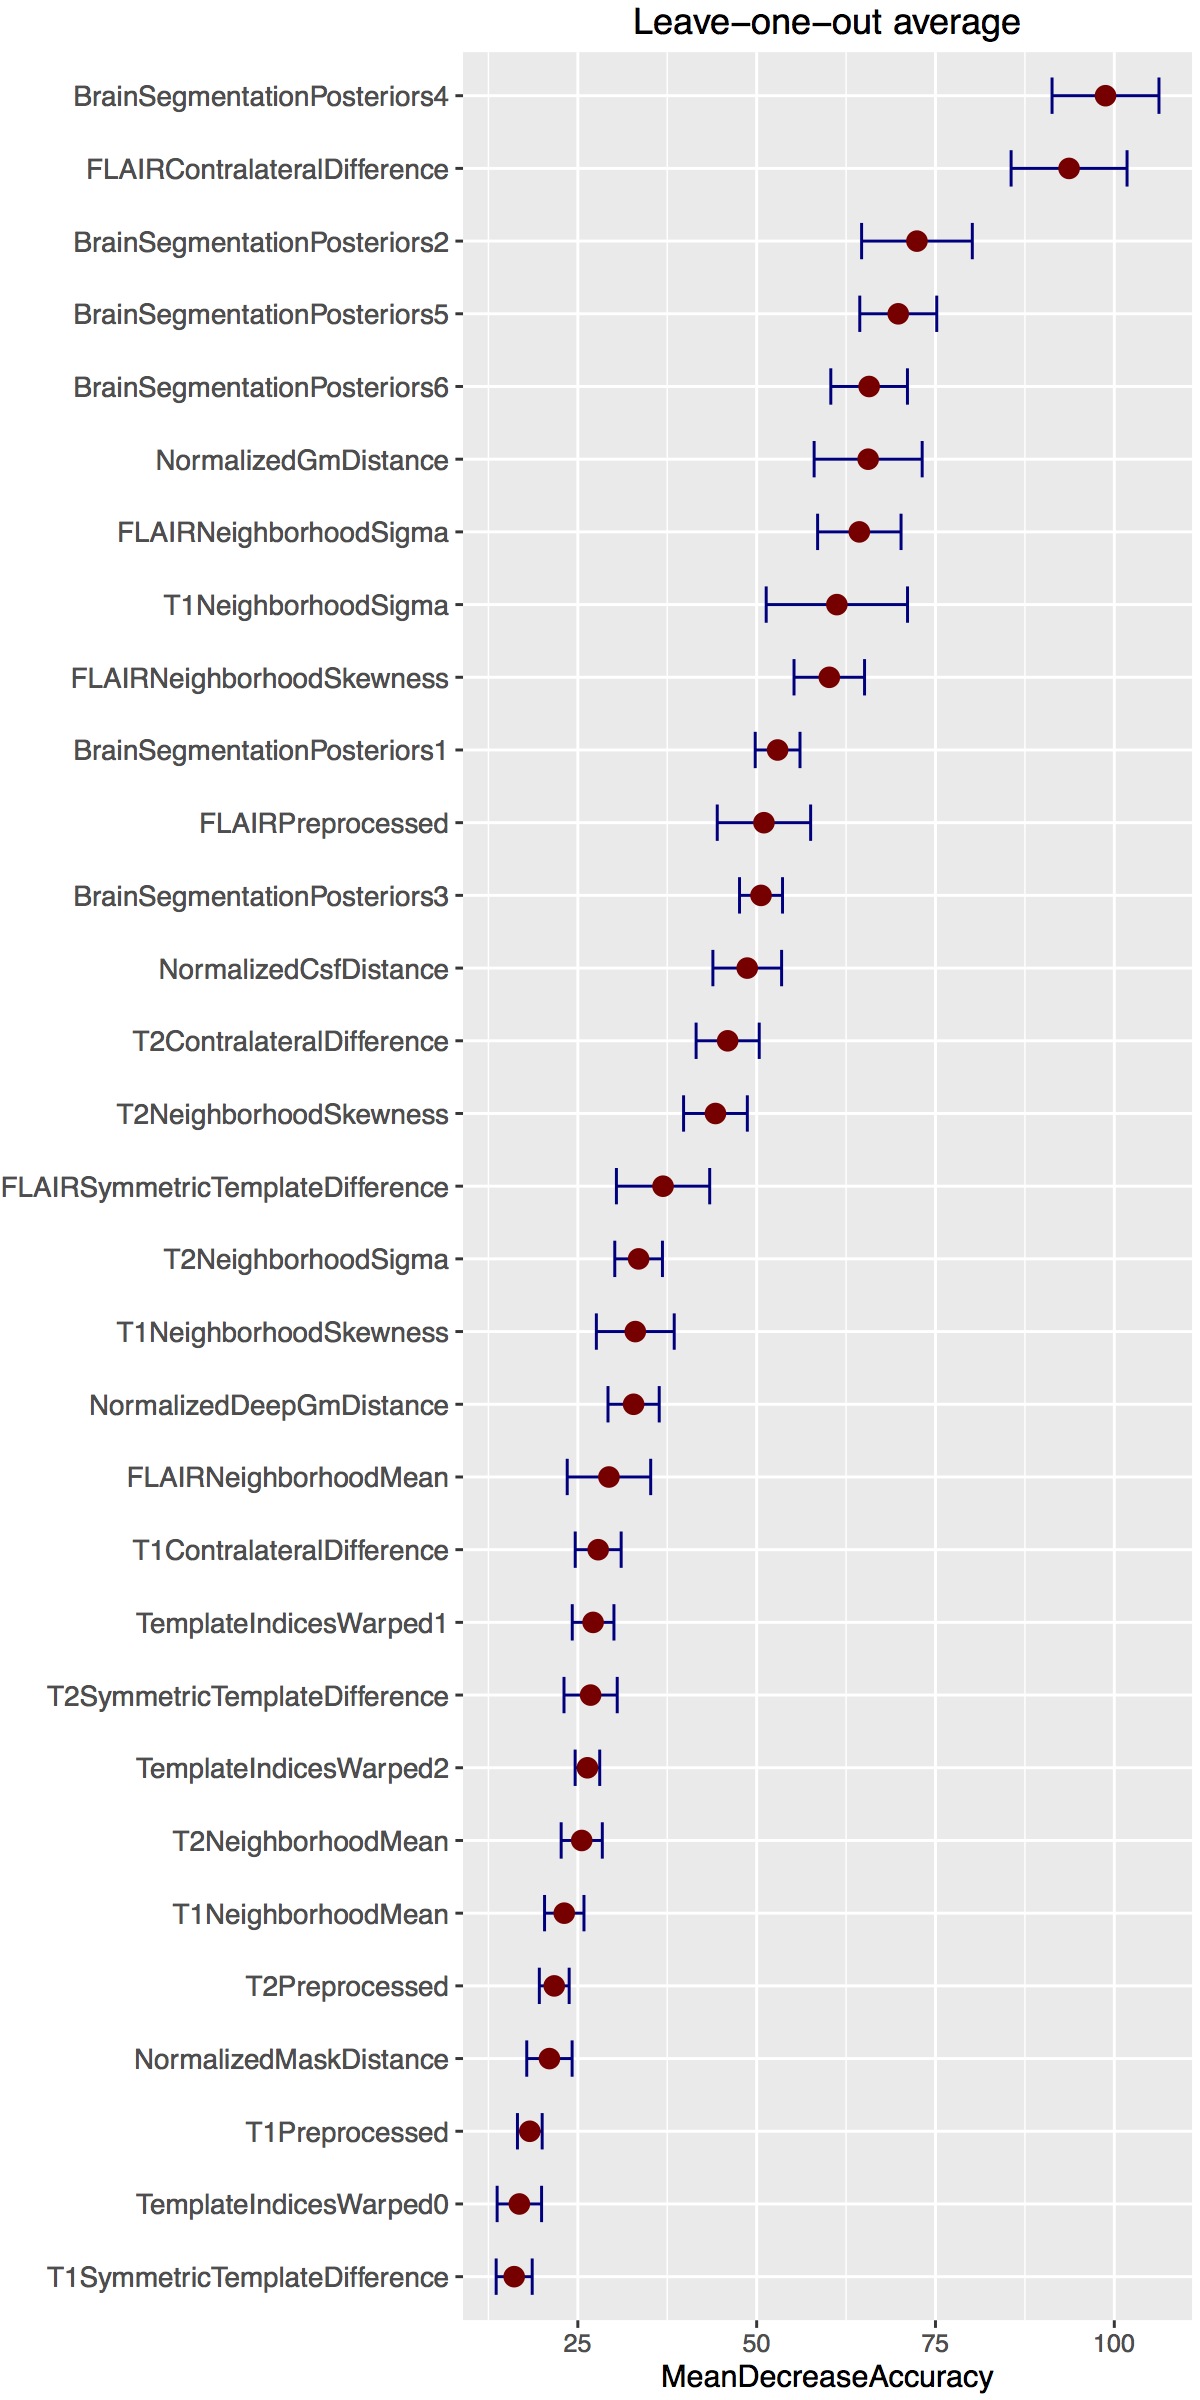
\includegraphics{Figures/averageLeaveOneOutStage1.png}
\caption{Average \emph{MeanDecreaseAccuracy} plots generated from the
creation of all 24 random forest models for Stage 1 during the
leave-one-out evaluation. These plots are useful in providing a
quantitative assessment of the predictive importance of each feature.
Features are ranked in descending order of importance. The horizontal
error bars provide the \(95^{th}\) percentile and illustrate the
stability of the feature importance across the leave-one-out models. At
this initial stage only 31 features images are used.}
\end{figure}

\begin{figure}[htbp]
\centering
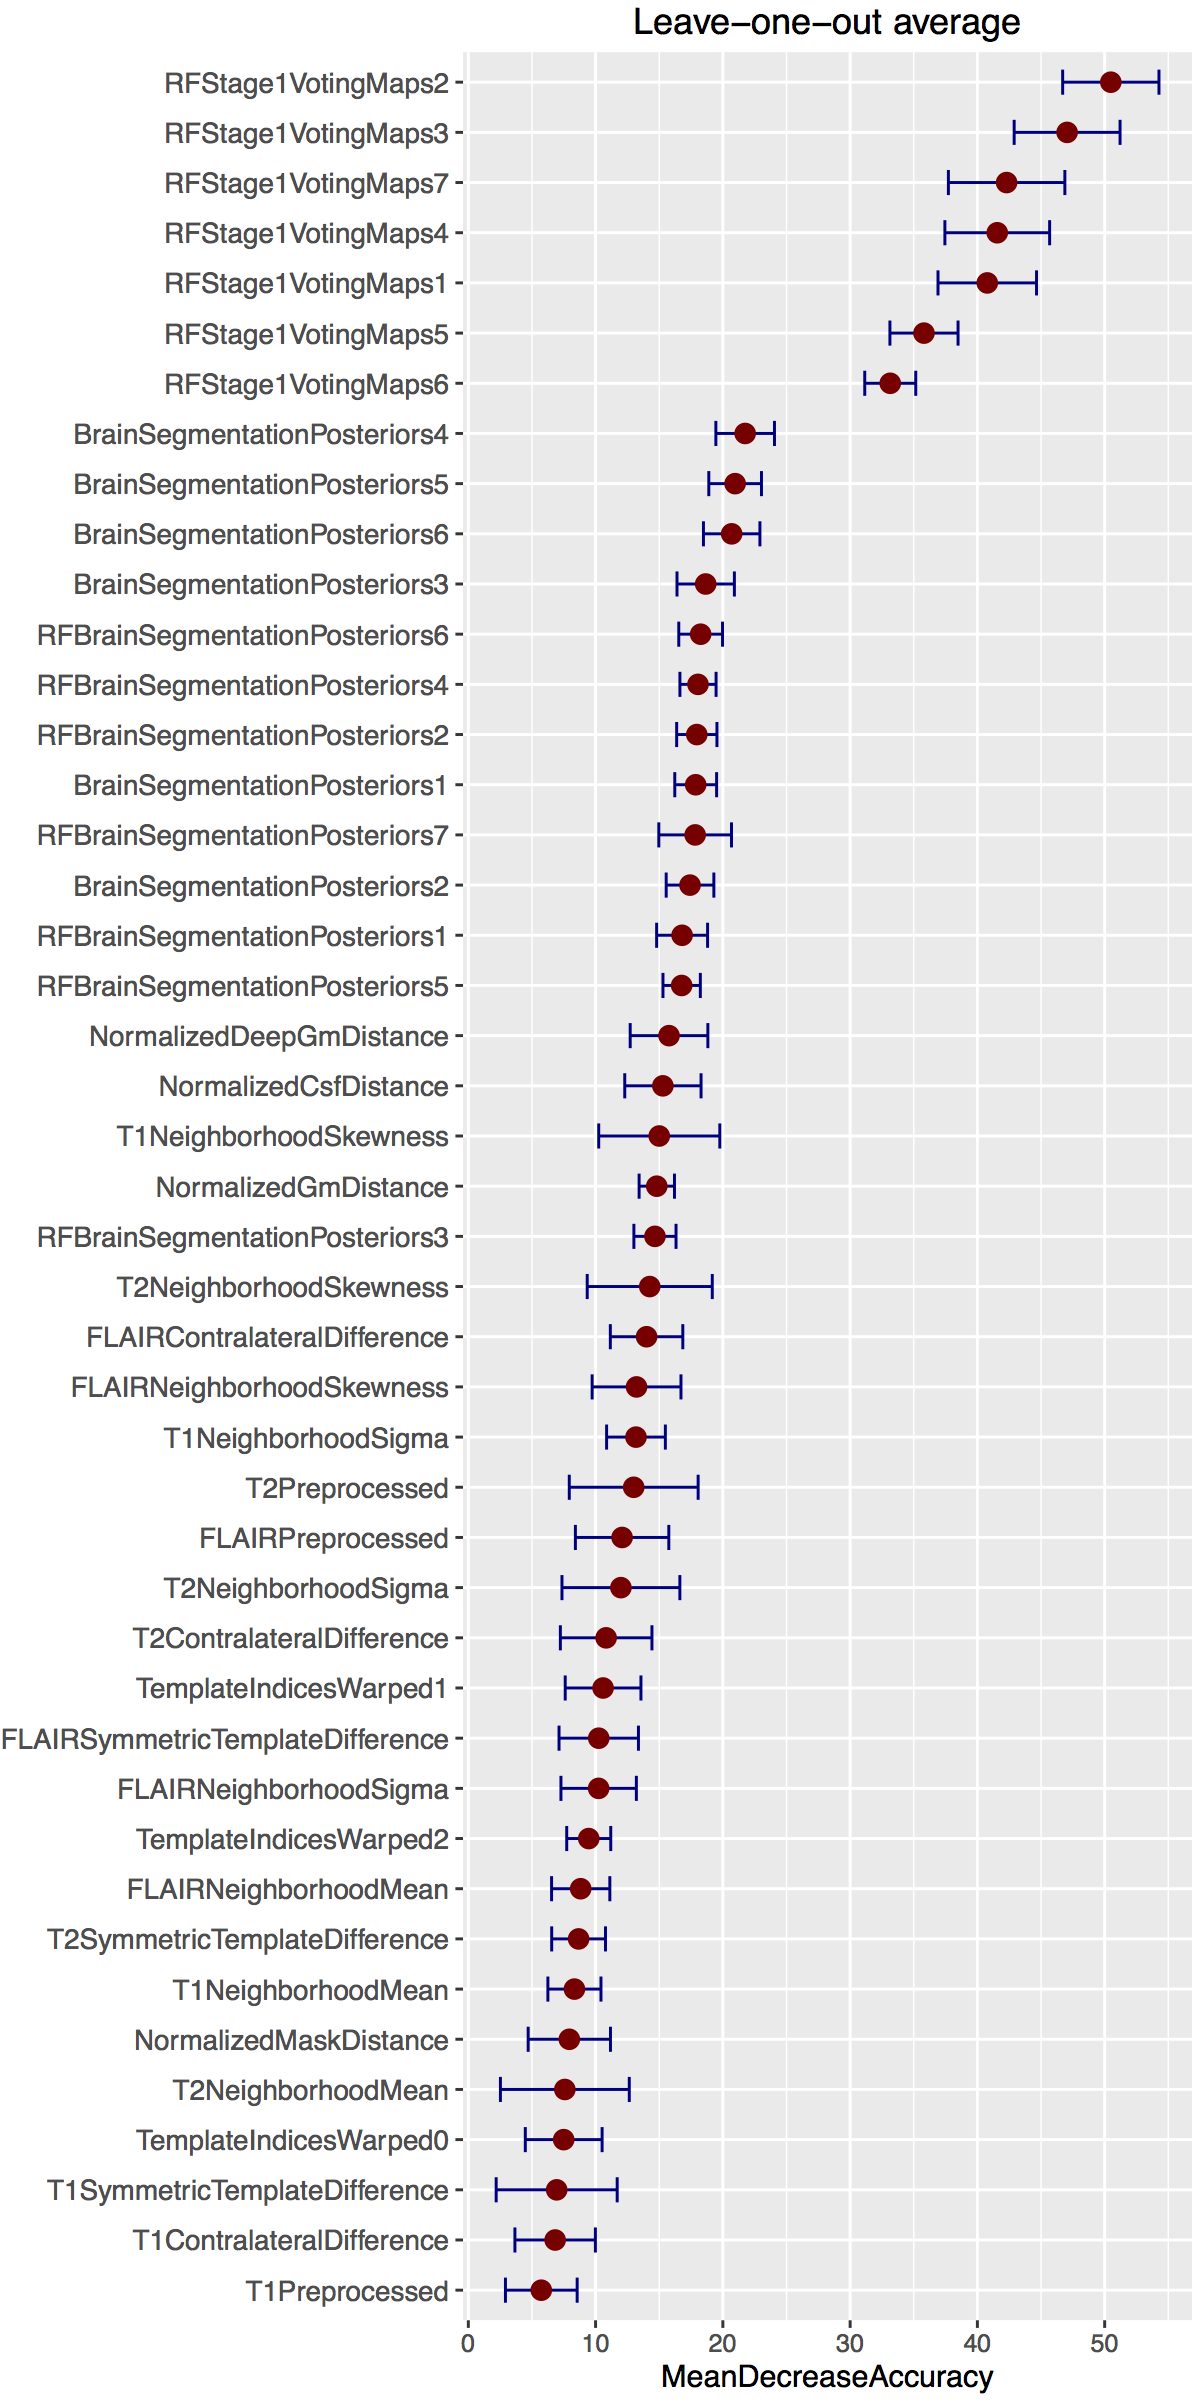
\includegraphics{Figures/averageLeaveOneOutStage2.png}
\caption{Average \emph{MeanDecreaseAccuracy} plots generated from the
creation of all 24 random forest models for Stage 2 during the
leave-one-out evaluation. These plots are useful in providing a
quantitative assessment of the predictive importance of each feature.
Features are ranked in descending order of importance. The horizontal
error bars provide the \(95^{th}\) percentile and illustrate the
stability of the feature importance across the leave-one-out models. We
augment the 31 feature images from the first stage by adding an
additional 7 voting maps and 7 segmentation posteriors from application
of the Bayesian-based segmentation for a total of 45 images for the
second stage.}
\end{figure}

The resulting rankings for both Stages are given in Figures 6 and 7
where the values for the separate stages are averaged over the entire
corresponding model set. In addition, we track the variance for each
feature over all models to illustrate the stability of the chosen
features during the evaluation. This latter information is illustrated
as horizontal errors bars providing the \(95^{th}\) percentile Note that
the reader can cross reference Table 1 for identifying corresponding
feature types and names.

\section{Discussion}\label{discussion}

\textcolor{blue}{
In evaluating the segmentation results, there are limited methodologies described in the
literature for automatic segmentation of WMHs despite the numerous clinical studies}\textsuperscript{39,40}
\textcolor{blue}{exploring the connections between WMHs and TBI.
However, we can extrapolate from similar application areas where such methodologies have a
much longer history of development such as white matter lesion segmentation in
multiple sclerosis )MS).  In a recent review [@Garcia-Lorenzo:2013aa], 47 total papers
were found during a literature search and evaluated which concern automated segmentation of white
matter lesions in MS.  The most widely-used data for algorithmic evaluation consists
of two cohorts from two different sites used in
the MS Lesion segmentation challenge associated with the international MICCAI 2008
conference.  For comparison, this challenge training data set
has a mean lesion load of 204 ($\pm$ 752) mm$^3$ per lesion (compared with
our mean lesion load of 33.8 ($\pm$ 55.4) voxels $\times$ 1.2 mm$^3$ per voxel =
40.56 ($\pm$ 66.48) mm$^3$ per lesion) and the resolution is
almost twice what is used in this study (i.e., 0.5 $\times$ 0.5 $\times$ 0.5).
Note that our relative volume difference numbers are comparable to the
relative volume difference {\em between raters} of 68 percent (cf Figure 5 (d))}\textsuperscript{41}.

Regarding the feature rankings, it is interesting to note some of the
other top performing features for Stage 1. The contralateral difference
FLAIR image is highly discriminative over the set of evaluation random
forest models (see Figure 8). This accords with the known clinical
relevance of FLAIR images for identifying white matter hyperintensities
and the fact that such pathology does not typically manifest
symmetrically in both hemispheres. Interestingly, the posterior maps for
the deep gray matter are extremely important for accurate white matter
hyperintensity segmentation. Perhaps the spatial specification of deep
gray matter aids in the removal of false positives. Inspection of the
bottom of the plots demonstrates the lack of discriminating features
associated with the T1 image which is also well-known in the clinical
literature.

\begin{figure}[htbp]
\centering
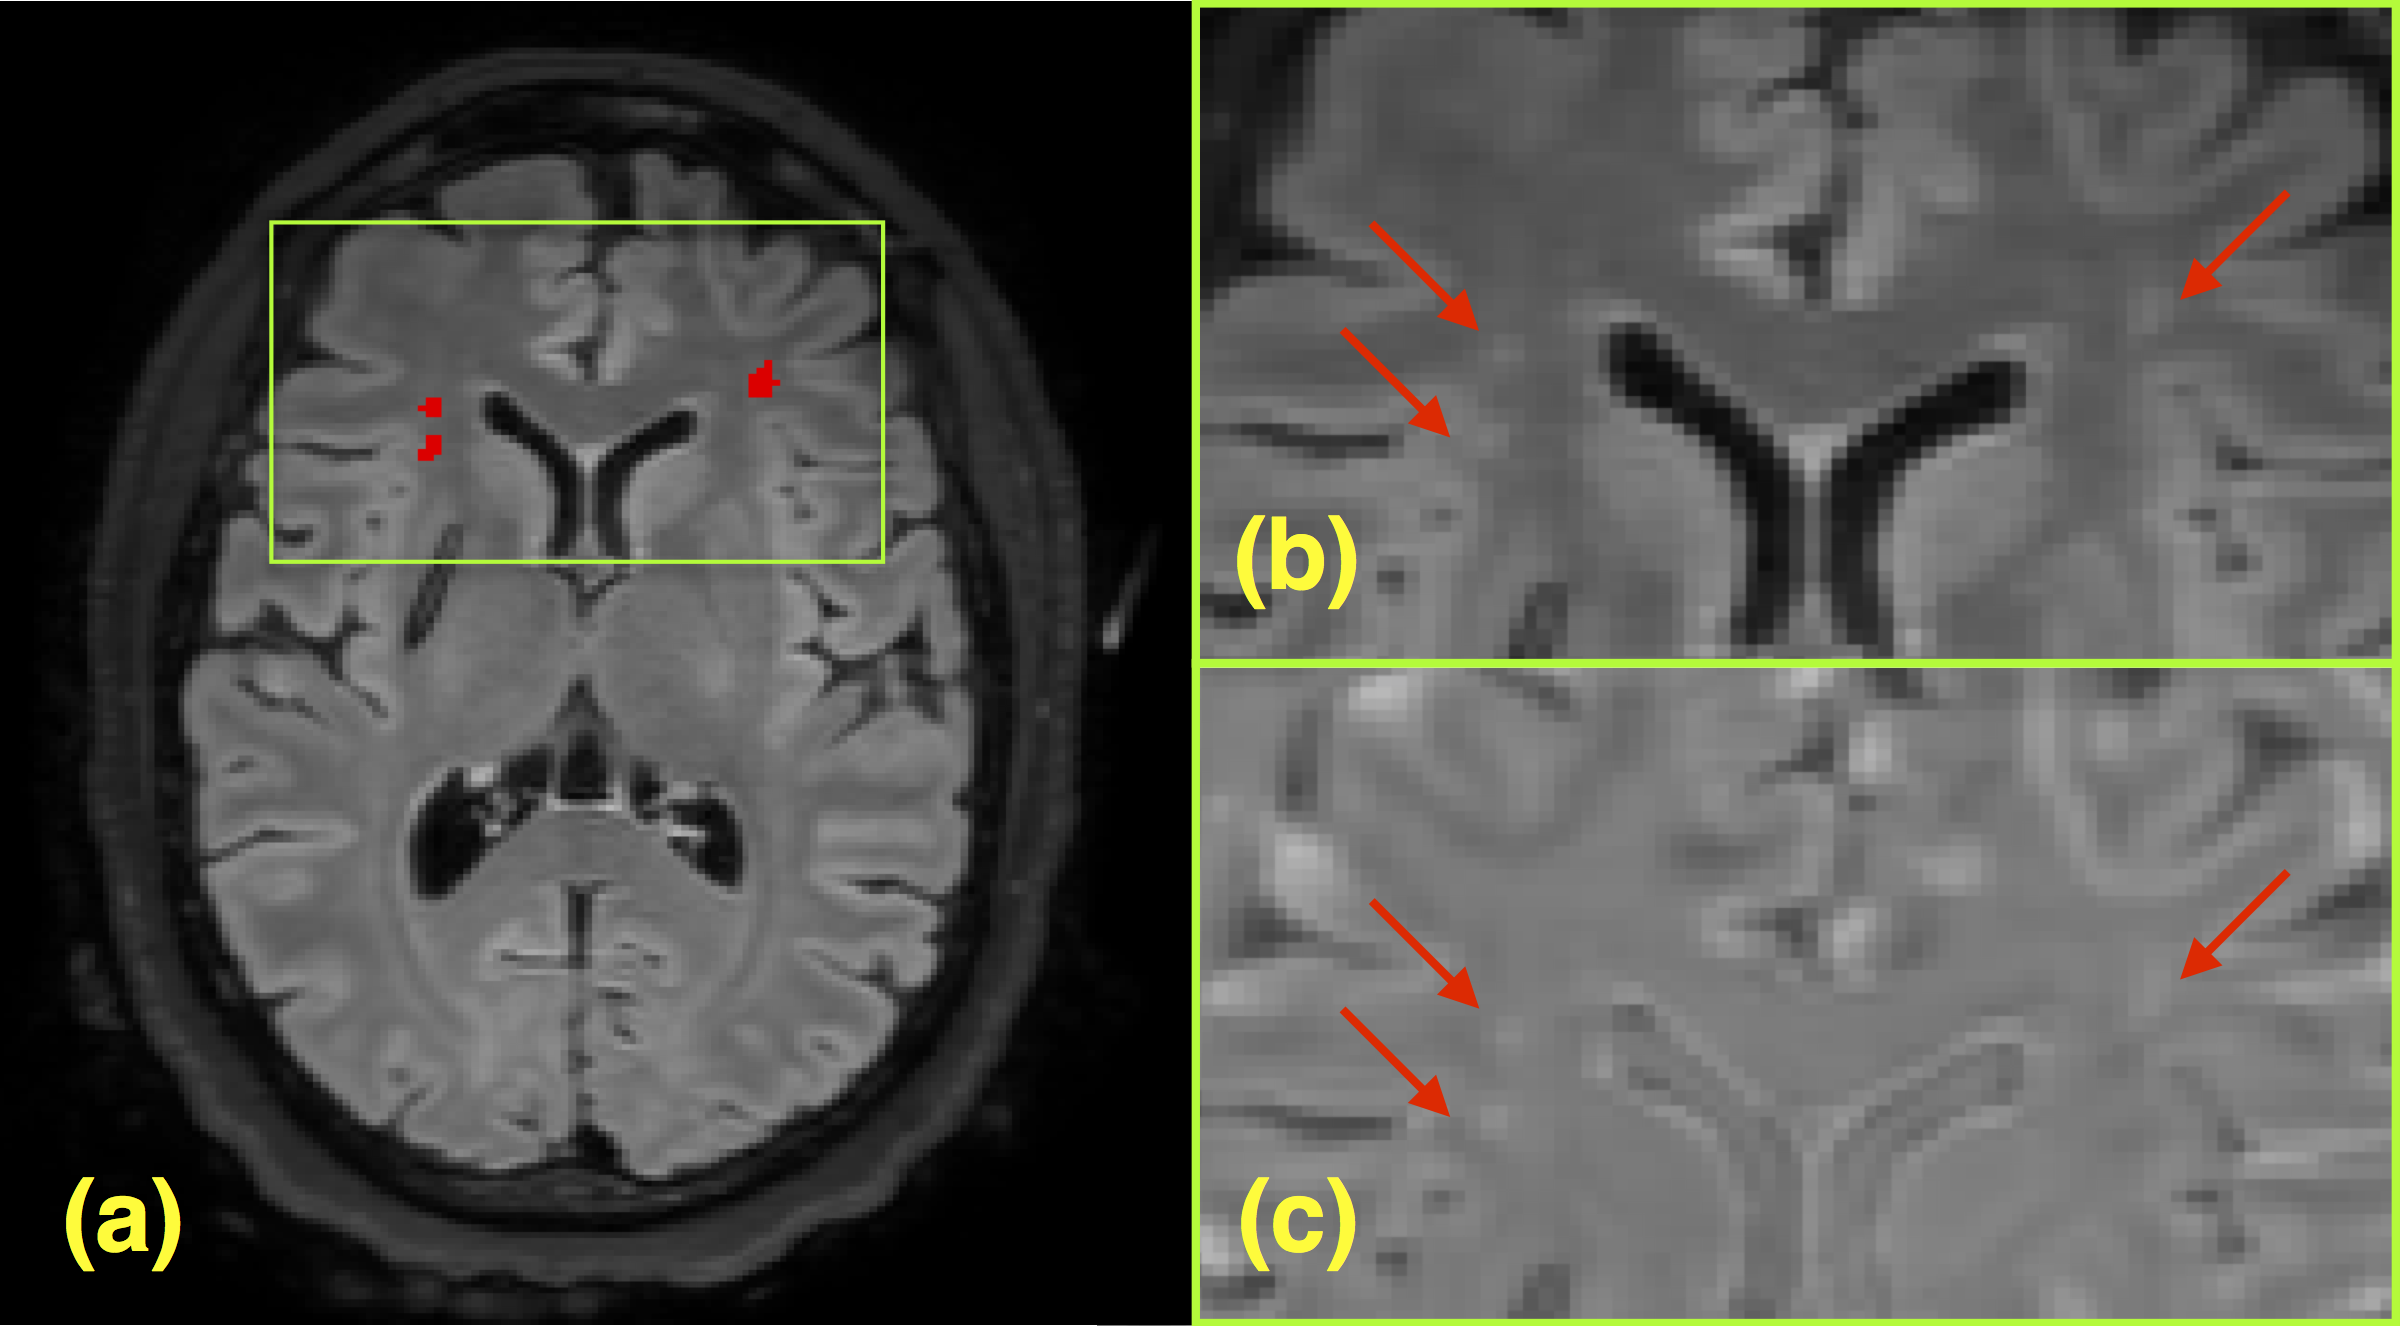
\includegraphics{Figures/FLAIRcontralaleteralWithLesionsAlternate.png}
\caption{(a) FLAIR image slice illustrating WMHs which have been
manually delineated. The region around the WMHs is enlarged (b) in the
original FLAIR and the (c) contralateral FLAIR difference image.}
\end{figure}

As described earlier, for Stage 2, we used the output random forest
voting maps from Stage 1 as both features themselves and as priors for
input to a Bayesian-based segmentation with an additional MRF spatial
prior. In Figure 7, the voting maps are labeled as
``\emph{RFStage1VotingMaps}'' where the final numeral is associated with
the brain parenchymal labeling given previously. Similarly, the
additional RF prior segmentation feature probability maps are labeled as
``\emph{RFBrainSegmentationPosteriors}''. The Stage 2 feature importance
plot follows similar trends as that for Stage 1 with the T1 images not
contributing much to the identification of white matter hyperintensity
voxels. The initial voting maps from Stage 1 are extremely important
with the top 3 being the estimated locations of the 1) gray matter, 2)
white matter, and 3) white matter hyperintensities. Since these tissue
type can be conflated based on intensity alone it is intuitive that such
features would be important.

\section{Conclusions}\label{conclusions}

The current communications describes a supervised statistical learning
methodology for identifying WHMs within multimodal MR brain imaging.
This effort utilized information acquired from the manual segmentation
of WMHs from FLAIR images to help build two-stage ensembles of decision
trees for the automated identification of these lesions. Although only a
single expert was used to produce the manual labelings, our intent is to
further refine the proposed paradigm by crowdsourcing with feedback from
other experts who interact with both the data and methodology. Also, we
recognize that only a single site was used for evaluating the proposed
framework. However, we are currently processing other site data with the
models developed for this work and the results look promising since the
developed features are site-agnostic.

As far as we know, this is the first report utilizing a novel random
forest approach to identify WMHs in a cohort of TBI patients. TBI WMHs
tend to be more difficult to segment than MS lesions as the former tend
to be smaller with an overall smaller lesion load. Also, enhancement
protocols with the former tend to be less successful than with the
latter. As mentioned previously, the work in MS lesion segmentation is
extensive with a handful of techniques being publicly available.

Two major meta-analyses of WMHs have been published covering the periods
prior to\textsuperscript{39} and after 2010\textsuperscript{40}. Debette
\& Markus\textsuperscript{39} found that the presence of WMHs was
related to subsequent cognitive decline, a higher risk of developing
dementia, stroke, and of mortality. Lesion volume at baseline was also
predictive of cognitive decline. Kloppenborg et al.\textsuperscript{40}
of 23 cross-sectional studies reporting MRI and concurrent
neuropsychological results in patients with heterogeneous diagnoses but
without previously diagnosed cognitive impairment, found that WMHs were
associated with cognitive deficit (effect size of -0.10, 95\% CI: -0.13
to -0.08) after controlling for age.

Despite the potential clinical significance of WMHs these lesions
receive little attention in current clinical workflows. When reported in
a standard neuroradiologist interpretation, they are typically handled
as incidental findings and are assigned little clinical significance.
This likely reflects the impracticality of performing a detailed
assessment of number, volume, and distribution within a qualitative
neuroradiologist interpretation as well as the lack of correlative
information on how the presence and distribution of these lesions may
inform a diagnosis and prognosis in the appropriate clinical setting. To
date, automated or semi-automated tools for the detection of WMHs have
lacked the specificity and efficiency for the mining of large-scale
datasets to generate highly granular data on whether these lesions
possess any true diagnostic or prognostic value in the setting of a
specific disease process. The present communication describes a
supervised statistical learning tool that is appropriate for the
application to such large-scale datasets.

\clearpage

\subsection{Acknowledgements}\label{acknowledgements}

The authors wish to acknowledge all other members of the CENC
Neuroimaging Steering Committee and CENC leadership (Drs. David X. Cifu,
Ramon Diaz-Arrastia, and Rick Williams) for their support. We also
gratefully acknowledge the assistance of Tracy Nolen, Chris Siege and
Kevin Wilson. We would also like to thank the study participants and
their family members. This project was jointly supported by the
Department of Defense (W81XWH-13-2-0095), the U.S. Department of
Veterans Affairs (I01 CX001135 and I01 RX 002174), as well as USUHS
Grant HU 0001-08-0001.

\subsection{Declaration of
Interest/Disclaimer}\label{declaration-of-interestdisclaimer}

The authors report no financial disclosures or conflicts of interest.
The views expressed here are those of the authors and do not necessarily
reflect the official policy of position of the Department of the Navy,
Department of Defense, nor the U.S. Government. This work was prepared
as a part of official duties; Title 17 USC §105 provides that Copyright
protection under this title is not available for any work of the U.S.
Government. Title 17 USC §101 defines a US Government work as a work
prepared by a military service member of employee of the US Government
as part of that person's official duties.

\clearpage

\section*{References}\label{references}
\addcontentsline{toc}{section}{References}

\hypertarget{refs}{}
\hypertarget{ref-Bigler:2013aa}{}
1. Bigler ED, Abildskov TJ, Petrie J, Farrer TJ, Dennis M, Simic N,
Taylor HG, Rubin KH, Vannatta K, Gerhardt CA, et al. Heterogeneity of
brain lesions in pediatric traumatic brain injury. Neuropsychology.
2013;27(4):438--51.

\hypertarget{ref-Smitherman:2016aa}{}
2. Smitherman E, Hernandez A, Stavinoha PL, Huang R, Kernie SG,
Diaz-Arrastia R, Miles DK. Predicting outcome after pediatric traumatic
brain injury by early magnetic resonance imaging lesion location and
volume. J Neurotrauma. 2016;33(1):35--48.

\hypertarget{ref-Marquez-de-la-Plata:2007aa}{}
3. Marquez de la Plata C, Ardelean A, Koovakkattu D, Srinivasan P,
Miller A, Phuong V, Harper C, Moore C, Whittemore A, Madden C, et al.
Magnetic resonance imaging of diffuse axonal injury: Quantitative
assessment of white matter lesion volume. J Neurotrauma.
2007;24(4):591--8.

\hypertarget{ref-Moen:2014aa}{}
4. Moen KG, Brezova V, Skandsen T, Håberg AK, Folvik M, Vik A. Traumatic
axonal injury: The prognostic value of lesion load in corpus callosum,
brain stem, and thalamus in different magnetic resonance imaging
sequences. J Neurotrauma. 2014;31(17):1486--96.

\hypertarget{ref-Ding:2008aa}{}
5. Ding K, Marquez de la Plata C, Wang JY, Mumphrey M, Moore C, Harper
C, Madden CJ, McColl R, Whittemore A, Devous MD, et al. Cerebral atrophy
after traumatic white matter injury: Correlation with acute neuroimaging
and outcome. J Neurotrauma. 2008;25(12):1433--40.

\hypertarget{ref-Pierallini:2000aa}{}
6. Pierallini A, Pantano P, Fantozzi LM, Bonamini M, Vichi R, Zylberman
R, Pisarri F, Colonnese C, Bozzao L. Correlation between mRI findings
and long-term outcome in patients with severe brain trauma.
Neuroradiology. 2000;42(12):860--7.

\hypertarget{ref-Weiss:2008aa}{}
7. Weiss N, Galanaud D, Carpentier A, Tezenas de Montcel S, Naccache L,
Coriat P, Puybasset L. A combined clinical and mRI approach for outcome
assessment of traumatic head injured comatose patients. J Neurol.
2008;255(2):217--23.

\hypertarget{ref-Levin:1988aa}{}
8. Levin HS, Williams D, Crofford MJ, High WM Jr, Eisenberg HM, Amparo
EG, Guinto FC Jr, Kalisky Z, Handel SF, Goldman AM. Relationship of
depth of brain lesions to consciousness and outcome after closed head
injury. J Neurosurg. 1988;69(6):861--6.

\hypertarget{ref-breiman2001}{}
9. Breiman L. Random forests. In: Machine learning. 2001. pp. 5--32.

\hypertarget{ref-yi2009}{}
10. Yi Z, Criminisi A, Shotton J, Blake A. Discriminative, semantic
segmentation of brain tissue in MR images. Med Image Comput Comput
Assist Interv. 2009;12(Pt 2):558--65.

\hypertarget{ref-viola2005}{}
11. Viola P, Jones M, Snow D. Detecting pedestrians using patterns of
motion and appearance. International Journal of Computer Vision.
2005;63:153--161.

\hypertarget{ref-geremia2011}{}
12. Geremia E, Clatz O, Menze BH, Konukoglu E, Criminisi A, Ayache N.
Spatial decision forests for MS lesion segmentation in multi-channel
magnetic resonance images. Neuroimage. 2011;57(2):378--90.

\hypertarget{ref-Pustina:2016aa}{}
13. Pustina D, Coslett HB, Turkeltaub PE, Tustison N, Schwartz MF,
Avants B. Automated segmentation of chronic stroke lesions using lINDA:
Lesion identification with neighborhood data analysis. Hum Brain Mapp.
2016 Jan.

\hypertarget{ref-geremia2012}{}
14. Geremia E, Menze BH, Ayache N. Spatial decision forests for glioma
segmentation in multi-channel MR images. In: Proceedings of MICCAI-BRATS
2012. 2012.

\hypertarget{ref-bauer2012}{}
15. Bauer S, Fejes T, Slotboom J, Wiest R, Nolte L-P, Reyes M.
Segmentation of brain tumor images based on integrated hierarchical
classification and regularization. In: Proceedings of MICCAI-BRATS 2012.
2012. pp. 10--13.

\hypertarget{ref-zikic2012}{}
16. Zikic D, Glocker B, Konukoglu E, Shotton J, Criminisi A, Ye DH,
Demiralp C, Thomas OM, Das T, Jena R, et al. Context-sensitive
classification forests for segmentation of brain tumor tissues. In:
Proceedings of MICCAI-BRATS 2012. 2012. pp. 1--9.

\hypertarget{ref-Tustison:2015aa}{}
17. Tustison NJ, Shrinidhi KL, Wintermark M, Durst CR, Kandel BM, Gee
JC, Grossman MC, Avants BB. Optimal symmetric multimodal templates and
concatenated random forests for supervised brain tumor segmentation
(simplified) with aNTsR. Neuroinformatics. 2015;13(2):209--25.

\hypertarget{ref-schapire1990}{}
18. Schapire R. The strength of weak learnability. Machine Learning.
1990;5:197--227.

\hypertarget{ref-freund1997}{}
19. Freund Y, Schapire R. A decision-theoretic generalization of on-line
learning and an application to boosting. Journal of Computer and System
Sciences. 1997;55:119--139.

\hypertarget{ref-ho1995}{}
20. Ho TK. Random decision forests. In: Document analysis and
recognition, 1995., proceedings of the third international conference
on. Vol. 1. 1995. pp. 278--282 vol.1.

\hypertarget{ref-amit1997}{}
21. Amit Y, Geman D. Shape quantization and recognition with randomized
trees. Neural Computation. 1997;9:1545--1588.

\hypertarget{ref-Avants:2014aa}{}
22. Avants BB, Tustison NJ, Stauffer M, Song G, Wu B, Gee JC. The
Insight ToolKit image registration framework. Front Neuroinform.
2014;8:44.

\hypertarget{ref-Yushkevich:2006aa}{}
23. Yushkevich PA, Piven J, Hazlett HC, Smith RG, Ho S, Gee JC, Gerig G.
User-guided 3D active contour segmentation of anatomical structures:
Significantly improved efficiency and reliability. Neuroimage.
2006;31(3):1116--28.

\hypertarget{ref-Tustison:2014ab}{}
24. Tustison NJ, Cook PA, Klein A, Song G, Das SR, Duda JT, Kandel BM,
Strien N van, Stone JR, Gee JC, et al. Large-scale evaluation of aNTs
and freeSurfer cortical thickness measurements. Neuroimage.
2014;99:166--79.

\hypertarget{ref-landman2011}{}
25. Landman BA, Huang AJ, Gifford A, Vikram DS, Lim IAL, Farrell JAD,
Bogovic JA, Hua J, Chen M, Jarso S, et al. Multi-parametric neuroimaging
reproducibility: A 3-T resource study. Neuroimage. 2011;54(4):2854--66.

\hypertarget{ref-Avants:2010aa}{}
26. Avants BB, Yushkevich P, Pluta J, Minkoff D, Korczykowski M, Detre
J, Gee JC. The optimal template effect in hippocampus studies of
diseased populations. Neuroimage. 2010;49(3):2457--66.

\hypertarget{ref-Neema:2009aa}{}
27. Neema M, Guss ZD, Stankiewicz JM, Arora A, Healy BC, Bakshi R.
Normal findings on brain fluid-attenuated inversion recovery mR images
at 3T. AJNR Am J Neuroradiol. 2009;30(5):911--6.

\hypertarget{ref-Tustison:2010ac}{}
28. Tustison NJ, Avants BB, Cook PA, Zheng Y, Egan A, Yushkevich PA, Gee
JC. N4ITK: Improved N3 bias correction. IEEE Trans Med Imaging.
2010;29(6):1310--20.

\hypertarget{ref-Manjon:2010aa}{}
29. Manjón JV, Coupé P, Martí-Bonmatí L, Collins DL, Robles M. Adaptive
non-local means denoising of mR images with spatially varying noise
levels. J Magn Reson Imaging. 2010;31(1):192--203.

\hypertarget{ref-nyul2000}{}
30. Nyúl LG, Udupa JK, Zhang X. New variants of a method of MRI scale
standardization. IEEE Trans Med Imaging. 2000;19(2):143--50.

\hypertarget{ref-Avants:2011aa}{}
31. Avants BB, Tustison NJ, Wu J, Cook PA, Gee JC. An open source
multivariate framework for \(n\)-tissue segmentation with evaluation on
public data. Neuroinformatics. 2011;9(4):381--400.

\hypertarget{ref-Menze:2015aa}{}
32. Menze BH, Jakab A, Bauer S, Kalpathy-Cramer J, Farahani K, Kirby J,
Burren Y, Porz N, Slotboom J, Wiest R, et al. The multimodal brain tumor
image segmentation benchmark (bRATS). IEEE Trans Med Imaging.
2015;34(10):1993--2024.

\hypertarget{ref-maurer2003}{}
33. Maurer CR, Rensheng Q, Raghavan V. A linear time algorithm for
computing exact Euclidean distance transforms of binary images in
arbitrary dimensions. Pattern Analysis and Machine Intelligence, IEEE
Transactions on. 2003;25(2):265--270.

\hypertarget{ref-Anbeek:2004aa}{}
34. Anbeek P, Vincken KL, Osch MJP van, Bisschops RHC, Grond J van der.
Probabilistic segmentation of white matter lesions in mR imaging.
Neuroimage. 2004;21(3):1037--44.

\hypertarget{ref-Tustison:2013ac}{}
35. Tustison NJ, Avants BB. Explicit B-spline regularization in
diffeomorphic image registration. Front Neuroinform. 2013;7:39.

\hypertarget{ref-Avants:2011ab}{}
36. Avants BB, Tustison NJ, Song G, Cook PA, Klein A, Gee JC. A
reproducible evaluation of ANTs similarity metric performance in brain
image registration. Neuroimage. 2011;54(3):2033--44.

\hypertarget{ref-Garcia-Lorenzo:2013aa}{}
37. García-Lorenzo D, Francis S, Narayanan S, Arnold DL, Collins DL.
Review of automatic segmentation methods of multiple sclerosis white
matter lesions on conventional magnetic resonance imaging. Med Image
Anal. 2013;17(1):1--18.

\hypertarget{ref-liaw2002}{}
38. Liaw A, Wiener M. Classification and regression by randomForest. R
News. 2002;2/3:18--22.

\hypertarget{ref-Debette:2010aa}{}
39. Debette S, Markus HS. The clinical importance of white matter
hyperintensities on brain magnetic resonance imaging: Systematic review
and meta-analysis. BMJ. 2010;341:c3666.

\hypertarget{ref-Kloppenborg:2014aa}{}
40. Kloppenborg RP, Nederkoorn PJ, Geerlings MI, Berg E van den.
Presence and progression of white matter hyperintensities and cognition:
A meta-analysis. Neurology. 2014;82(23):2127--38.

\hypertarget{ref-vanginneken:2007aa}{}
41. Ginneken BV, Heimann T, Styner M. 3D segmentation in the clinic: A
grand challenge. In: 3D segmentation in the clinic: A grand challenge.
2007. pp. 7--15.

\end{document}
